\documentclass[10pt,conference,compsocconf,letterpaper]{IEEEtran}
\makeatletter
\def\ps@headings{%
\def\@oddhead{\mbox{}\scriptsize\rightmark \hfil \thepage}%
\def\@evenhead{\scriptsize\thepage \hfil \leftmark\mbox{}}%
\def\@oddfoot{}%
\def\@evenfoot{}}
\makeatother
\pagestyle{headings}

\usepackage{amsmath,amsfonts}
\usepackage{times,epsfig,endnotes,color,url,paralist, multirow}
\usepackage[lined,ruled,linesnumbered,vlined]{algorithm2e}
\IEEEoverridecommandlockouts

\begin{document}
\pagestyle{empty}
\title{DMap: A Shared Hosting Scheme for \\ Dynamic Identifier to
  Locator Mappings \\ in the Global Internet$^{\star}$
\thanks{$^{\star}$This research was supported in part by NSF Future Internet Architecture (FIA) grant CNS-1040735.}
}

\author{Tam Vu\authorrefmark{1},
    Akash Baid\authorrefmark{1},
    Yanyong Zhang\authorrefmark{1},
    Thu D. Nguyen\authorrefmark{2}, \\
    Junichiro Fukuyama\authorrefmark{3},
    Richard P. Martin\authorrefmark{1}\authorrefmark{2},
    Dipankar Raychaudhuri\authorrefmark{1}  \\ \\
   \authorrefmark{1}WINLAB, Rutgers University, {\em\{tamvu, baid, yyzhang, rmartin, ray\}@winlab.rutgers.edu}
  \\  \authorrefmark{2}Department of Computer Science, Rutgers University, {\em tdnguyen@cs.rutgers.edu}
  \\  \authorrefmark{3}Toyota InfoTechnology Center USA, {\em jfukuyama@us.toyota-itc.com }
}


\maketitle
\begin{abstract}
    %As more mobile devices are connected to Internet, separating host names from network addresses is becoming a key enabling technique. In this paper we propose a novel architecture to do fast naming resolution service that can provide the mapping from a host name to its network address, thus facilitating this separation. We take a distributed approach by storing the mappings on the routers, and uses consistent hashing to find the routers that store a specific host name. As a result, our naming resolution service is scalable, fast, and reliable. Through detailed simulations with *** routers and *** names, we show that we can achieve *** ms lookup latencies.
This paper presents the design and evaluation of a novel distributed shared hosting approach, DMap, for managing dynamic identifier to locator mappings in the global Internet.  DMap is the foundation for a fast global name resolution service necessary to enable emerging Internet services such as seamless mobility support, content delivery and cloud computing.
%The proposed global name resolution service (GNRS) supports mobility at-scale in the future Internet in which a clean separation of the ``name" of a network object from its ``address" takes place. The GNRS is intended as a fast network-level service which can be queried by both end-points and in-network routers in order to obtain bindings between a GUID (globally unique identifier for the name) and the current routable network address (or addresses).
Our approach distributes identifier to locator mappings among Autonomous Systems (ASs) by directly applying K$>$1 consistent hash functions on the identifier to produce network addresses of the AS gateway routers at which the mapping will be stored. This direct mapping technique leverages the reachability information of the underlying routing mechanism that is already available at the network layer, and achieves low lookup latencies through a single overlay hop without additional maintenance overheads. The proposed DMap technique is described in detail and specific design problems such as address space fragmentation, reducing latency through replication, taking advantage of spatial locality, as well as coping with inconsistent entries are addressed. Evaluation results are presented from a large-scale discrete event simulation of the Internet with $\sim$26,000 ASs using real-world traffic traces from the DIMES repository. The results show that the proposed method evenly balances storage load across the global network while achieving lookup latencies with a mean value of $\sim$50 ms and $95^{th}$ percentile value of $\sim$100 ms, considered adequate for support of dynamic mobility across the global Internet. 
\end{abstract}

\newcommand{\arcName}{DMap}

\section{Introduction}
%% {\bf [ID/Locator split is the way to solve 4 issues in current
%% Internet including routing scalability, mobility support,
%% multi-homing
%% support and traffic engineering enhancements]}
The concept of separating identifiers from routable addresses or locators has been advocated by a number of authors in the networking community~\cite{saltzer,bennett,moskowitz,milsa}.
%There is a long history in the networking community separating the binding between identifier names and addresses -- the network-attached object named in the communication is separate from the network structure.That is, the sources and destinations should not be implicitly or explicitly bound to the network topology.
Separation of names from addresses makes it possible to avoid implicit or explicit binding of sources and destinations to the network's actual topology. 
Using existing terminology, the {\em identifier} names a
communicating object, such as a particular mobile phone, while the {\em locator}
identifies an address the network can use to route messages. For example,
a phone connecting to different 3G, 4G, and WiFi networks would get a separate
locator for each network. However, the identifier,
which in this case could be the International Mobile Subscriber Identity (IMSI) number, would remain the same. The goal of this work is to explore the
feasibility of identifier based communication under the assumption of large-scale dynamic mobility of named objects. In the above example, programmers should be able to send messages to a particular phone based on its IMSI number rather than to
an IP address. We take the position that identifiers can also be used to name
abstract entities and services; they need not to be tied to a particular
device. %However, the identifier should not be bound to any particular
%network topology.

%%{\em \bf why are global IDs good?}
Identifier based communication has many advantages, including simplified implementation session management, multi-homing, mobility, disconnection, authentication and
security~\cite{saltzer,bennett,moskowitz,milsa}.
When there is a high degree of dynamism between the communicating entities
and the network (as in most mobile service, content retrieval and cloud computing scenarios), using identifiers  to define network-attached objects is more appropriate than using locators.
Intuitively, it is easier to work with networking primitives based on identifiers when the locator changes faster than the
timescales of the communication session. For example, a voice call may last 30 minutes,
but a mobile device in a vehicle may change its network attachment points
many times during this period.

%%Requiring application developers to manage
%%variable and missing locators places an
%%undue burden on them compared to
%%expressing identity and then having the network manage the locators.
%%In addition, expressing identity allows the re-use of
%%the management software across many applications.
%%Finally, expressing identifiers allows the possibility of the
%%network using them for routing, buffering and authentication as well.

%%{\em \bf what we are doing an why it is hard about this:}

%%In this work we seek enabling technologies toward practical
%%implementation communications using global identifiers instead of
%%the current locator based approach, i.e., all
%% receiving messages based on global IDs rather than IP addresses.
Realizing an identifier based protocol stack has
several challenging aspects; the key design issue we address in this work is the
dynamic binding of identifiers to locators. That is, when the user presents
the networking stack with an identifier, the networking subsystem
must quickly return a set of locators, or {\em network addresses} (NAs)
back to the user. We address the challenge of providing a fast global name resolution service at Internet scale in this paper, and describe and evaluate a specific \textit{Direct Mapping (\textbf{DMap})} scheme for achieving a good balance between scalability, low update/query latency, consistency, availability and incremental deployment.

We take note of two trends in the Internet community that have significant bearing on the design of a global name resolution scheme. First, a flat identifier space is preferred to the hierarchical domain names currently used in the Internet. The use of flat, location independent identifiers is a central tenet of a number of clean slate proposals such as AIP~\cite{andersen}, HIP~\cite{moskowitz}, ROFL~\cite{CaesarRofl} and MobilityFirst~\cite{mobilityFirst}. The key advantage of flat labels lies in their use for direct verification of the binding between the name and an associated object (see~\cite{Ghodsi-ICN} for a detailed discussion).  As a result, name resolution schemes that rely on the hierarchical structure of the name such as the Domain Name System (DNS) or LISP-TREE~\cite{jakab} are not suitable for supporting such a flat identifier space.

The second trend is that due to its separation from the network attachment point, global names or identifiers will tend to belong to end-users or application providers rather than to the network, as is currently the case with IP. Hosts and other network-attached objects (content, computing services, etc.) are not owned by any Internet Service Provider (ISP), but they just happen to be connected to a particular Autonomous System (AS). Most name resolution schemes propose to store the mappings of the identifiers belonging to an AS inside that AS only~\cite{mathy}. The same rationale, however, does not work for a host-based identifier space because hosts (or content) do not belong to any particular AS, especially with the increasing number of mobile hosts which often have multiple simultaneous points of network attachment. Thus we challenge the assumed constraint of ownership based storage and design a scheme with network-wide sharing of the identifier-locator mappings independent of the AS boundaries.
 \begin{center}
        %\vspace{-0.2in}
        \begin{figure}[t]
            \centering           
            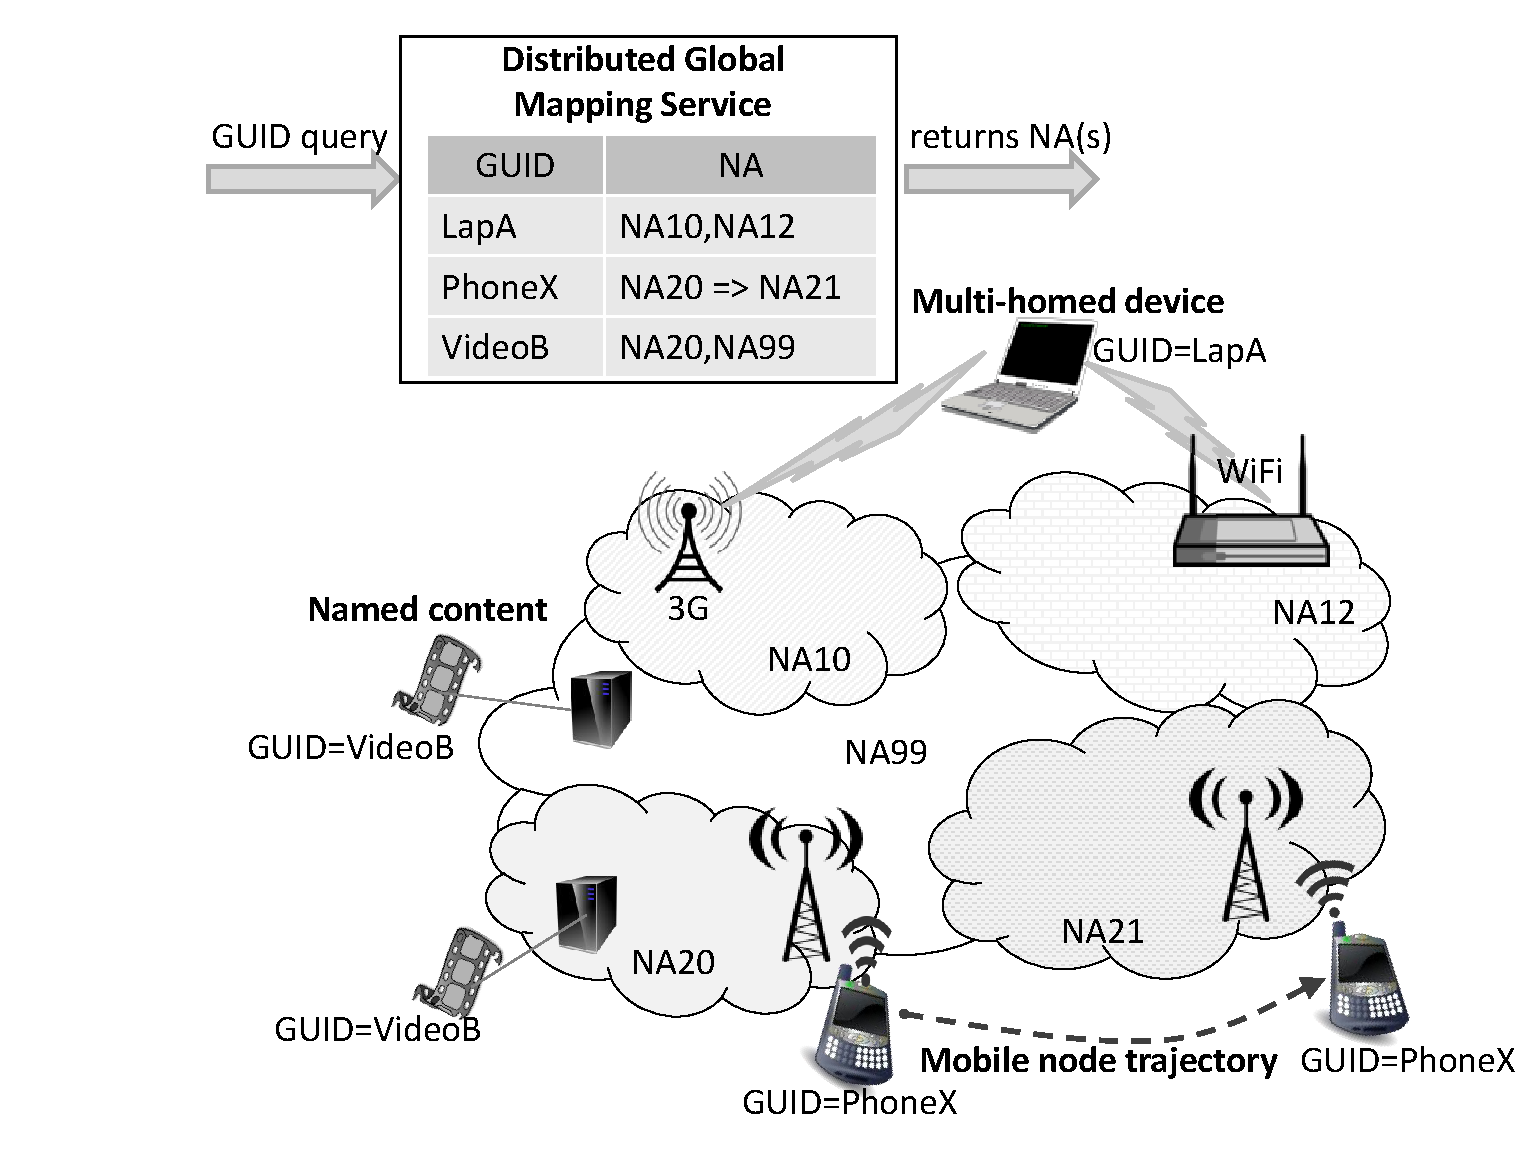
\includegraphics[ trim = 0.1in 0in 0in  0.1in, clip,width=0.5\textwidth]{figures/overview.eps}
            \vspace{-0.1in}
            \caption{Distributed global identifier to locator mapping service}
            \label{fig:overview}
			\vspace{-0.15in}
        \end{figure}

    \end{center} 
\vspace{-0.3in} 
% \hspace{0.1in}

Motivated by these trends, we propose a dynamic identifier to locator mapping management scheme called DMap which supports a flat space of a identifiers, referred to as {\em Globally Unique Identifiers}, or GUIDs. A GUID is a long bit sequence, such as a public key, that is globally unique and long enough that the chance of a collision is infinitesimally small. Each end host, such as laptops, mobile phones, servers and virtual machines can have a GUID. In addition, even abstract objects, such as a piece of content or a particular context, can have GUIDs. Each GUID is associated with one or more network addresses (NAs) that it attaches or belongs to. For example, the NAs of a multi-homed laptop in Figure~\ref{fig:overview} includes the NA of its 3G service provider and the NA of the network that its WiFi interface attaches to. We denote the identifier to locator mapping as the GUID$\rightarrow$NA mapping.

To perform the mapping service for a given GUID, DMap applies $K (K>1)$ hashing functions onto it to produce a list of $K$ network addresses, which are IP addresses in today's Internet, and stores the GUID$\rightarrow$NA mapping in the ASs that announce those network addresses. By doing so, DMap spreads the GUID$\rightarrow$NA mappings amongst ASs, such that an AS will host mappings of other ASs, as well as have its mappings hosted by others. A key advantage of this {\em shared hosting} approach is that it allows the hosting ASs to be deterministically and locally derived from the identifier by any network entity. DMap is simple yet efficient. It leverages the routing infrastructure to reach the hosting AS in a single overlay hop; it does not require a home agent, unlike mobile IP and existing cellular networks. Further, the potential shortcoming of the direct mapping scheme, lack of locality, is addressed by having multiple copies of the mappings that are stored in multiple locations. We further improve the design by including a local copy of the mapping within the AS that the GUID is residing in (this AS may change as the host moves).

Through detailed simulation studies, we show DMap achieves a $95^{th}$ percentile round trip query response time of below 100ms, which is important to support the fast growing class of mobile devices connected to the Internet.
%
%
%We set as a target the ability to
%support voice application under these conditions,
%with frequent handoffs. 
%Existing cellular telecommunication networks typically support handoffs within 100-200 ms~\cite{3gpp}. 
Our results also show that DMap can proportionally distribute GUID$\rightarrow$NA mappings among ASs, which is critical to scale our system to support billions of GUIDs and NAs associated with a global scale network. 
%
%shares the scalability goals of many other works, in that
%it should scale to billions of GUIDs and NAs. If we wish to use GUIDs
%as a replacement for mobile phone applications, we need to support
%this level of scale. 
%DMap's approach to scale is to leverage
%the number and sizes of the participating ASs.
%
%We found DMap can support such
%low latencies by showing it can update the GUID to locator mapping,
%e.g., GUID$\rightarrow$NA,
%in this regime. Using DMap for these applications also means that any
%inconsistencies can be resolve in sub-second timescales.


%%{\em \bf why our approach is novel, and our contributions}

%Our approach, called direct mapping (DMAP), is unique in several ways.
%First, rather than a completely new design, we seek to
%enable incremental deployment by leveraging the
%existing Internet routing framework as much as possible.
%Our approach builds on top of the routing tables created by
%the Border Gateway Protocol (BGP). The existing routing tables
%give us a partial view that greatly simplifies the design.

%Second, DMAP assumes a different fairness and trust model compared to
%previous works. In many identifier based approaches, each
%Autonomous System (AS) ownes a set of identifiers, and stores mappings
%between identifiers and locators for its identifier set.


%DMAP also introduces a new fairness metric. In many schemes, each
%hosting entity is considered equal. However, in DMAP's approach,
%each entity, in our case an AS, should host a number of mappings
%proportional to the amount of network address space they claim. That is,
%a large Internet Service Provider (ISP), with many ASes and claiming
%a lot of IP address space must host many more mappings than
%a small ISP with a small amount of address space. This is intuitively
%fair because large ISPs claiming large fractions of the IP address space
%should also have a large number of customers, and thus a large
%number of mappings.

%We found that shared hosting leads to drastically reduced mapping resolution
%latency compared to Distributed Hash Table (DHT)
%based schemes without requiring any Domain
%Name System (DNS) like infrastructure services. In addition, it allows us
%to use a flat identifier space. Unlike other hierarchical based global name
%spaces, such as DNS, DMAP supports a flat space of a identifiers, that is,
%identifiers with no internal hierarchical structure. We call these
%{\em Globally Unique Identifiers}, or GUIDs. A GUID is a long bit sequence,
%such as a public key, that is globally unique and long enough that the chance
%of an accidental collision is infinitesimally small.




%That is, the 100,000's of ASs should support several

%We evaluate DMap using a trace driven simulation approach.
%Using existing popularity models, we first simulate a binding service
%workload. We then evaluate the query latency given the
%real AS graph, considering actual hop counts and latency distributions.
%We demonstrate that DMap's shared hosting approach is feasible and gives
%good performance, under 100 ms latency in most cases. We show that
%DMap is robust to BGP churn and router failures. Finally, we present
%an analytic model that evaluates the expected AS hop-count and latency needed
%to perform the mappings. The analytic results are in agreement with
%the simulation results. The model shows that
%current trends in the Internet would lead to further improvements in DMap's performance.

The rest of paper is organized as follows. In Section~\ref{sec:overview}, we provide the background and motivation for DMap. The working of DMap and how DMap addresses several technical challenges are discussed in Section~\ref{sec:design}. We present detailed simulation evaluation results in Section~\ref{sec:evaluation}, and an analytical model in Section~\ref{sec:model}. Finally, we have the related work in Section~\ref{sec:related} and the concluding remarks in Section~\ref{sec:conclusion}.


%% {\bf Simple figure capturing use case of GNRS inserted here}

%\subsection{Key Contributions}

%The main contributions that we make in this paper are:

%Based on these requirements we introduce a mapping distribution scheme in which, instead of each AS storing and managing its set of identifier-locator tables, each mapping entry is managed by a set of foreign ASs. We explain the reasons behind this choice, point out its benefits and address the evident incentive and privacy issues. Specifically, our approach leverages the locator reachability information (IP reachability in the present Internet context) that is readily available at the network layer, and makes use of an in-network single hop hashing technique to reach the storage point for any given identifier-locator mapping entry with low latency. We make the following key contributions in this paper:

%\begin{enumerate}
%\item
%We propose a co-operative identifier to locator mapping scheme that
%distributes the mapping entries among participating ASs without regard
%to ownership and AS boundaries. We enumerate its benefits and address
%the evident problems associated.
%We propose a conceptual shift from ASs `owning' endpoint identifiers and individually storing the mappings of its owned set of identifiers to a network-wide sharing of the identifier-locator mappings irrespective of the AS boundaries. Our scheme results in a natural order of incentives in which an AS which is expected to produce a large number of identifier-locator lookups from other ASs, itself stores and answers a proportionally large number of mappings. We aim to provide reasonings that show the feasibility of the scheme in order to open further research into this line of thought.

%\item
%We introduce a novel single-hop hashing technique in
%Section~\ref{sec:design} that leverages the IP reachability
%information available at the network layer for low-latency mapping
%queries. To lookup a mapping in this scheme, one can directly hash the
%identifier to produce the network address of the AS that stores its
%mapping.

%\item
%We validate our scheme through a large-scale discrete event simulation
%based on Internet measurement traces. We show in
%Section~\ref{sec:evaluation} that this scheme achieves low latency
%values with a 95th percentile value of $\sim$100 ms, a 2x - 5x
%reduction compared to previously published results.

%\end{enumerate}


%% vassiliou_2009, 802.11 latencies of 200-400 ms
%% Mishra:2003:EAI:956981.956990, mean latencies of 3-4 seconds


%\section{Mapping identifiers to locators in mobile centric architecture}

In order to gain more insights into the requirements of the envisioned mapping scheme and highlight the difference in its usage compared to similar schemes for the LISP proposal, we provide a brief overview of the MobilityFirst architecture, enabling which is a key focus of the XYZ scheme. 

MobilityFirst is a `clean-slate' future Internet architecture project funded by the NSF FIA program~\cite{fia} with a particular focus on supporting large-scale, efficient and robust mobility services in the future Internet. The architecture is motivated by the dramatic growth of mobile devices and applications on the Internet and targets the projected dominance of mobile Internet traffic over that of fixed hosts in the near future~\cite{cisco-2010}. As depicted in Figure~\ref{fig:mobilityFirst} (reproduced from~\cite{nelson-11}), a central principle of the architecture is that every host has a permanent, location independent, globally unique identifier (GUID) which can then be mapped to a set of routable locators or network addresses (NA) corresponding to the current point(s) of attachment. In addition to hosts, GUIDs can refer to content and context to provide seamless content and context handling support in the future Internet. In terms of mapping scheme requirements, this leads to a much larger number of identifiers than the projected number of hosts usually considered in LISP based schemes. The MobilityFirst proposal includes late or repeated binding support, i.e., resolving a GUID to a network address at different points along the route in order to support rapid host mobility. This creates stricter latency requirements for the mapping lookups. Another aspect of the design which affects the mapping scheme is storage aware routing which gives routers the option to temporarily store data as a network-layer routing decision. Retransmitting the stored packets would require another mapping lookup leading to a much higher number of lookups compared to LISP based schemes.

    \begin{center}
        %\vspace{-0.2in}
        \begin{figure}[t]
            \centering
            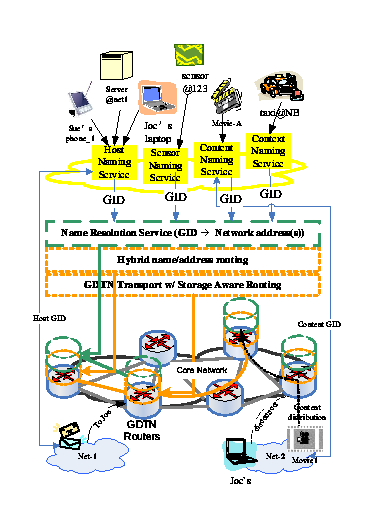
\includegraphics[width=0.8\textwidth]{figures/mobilityFirst.eps}
            \caption{Separation of identifiers (GUID) and locators (NA) in the MobilityFirst architecture}
            \label{fig:mobilityFirst}
        \end{figure}
    %\vspace{-0.2in}
    \end{center}

%\subsection{Why a new mapping Scheme? }
Why not MobileIP 
Comparing with other mapping scheme 

Given the number of identifier-locator mapping schemes recently proposed, the natural place to start is by exploring why we need a shift from traditional mechanisms. As Carpenter succinctly identified~\cite{carpenter}, the design of any mapping scheme which enables location/identifier separation in the future Internet depends on the implicit or explicit assumptions made on certain key issues - Should the scheme depend on the identifier space? What is the expected scale of identifier namespaces? Is the mapping invoked only upon the start of transmission or at successive domain boundaries while a packet is in-transit? What is the lifetime of a mapping? Should the scheme support dynamic identifier-locator mapping for mobility? and Does the mapping scheme have any impact on privacy? The design choices made by most of the existing proposals focus on a subset of these issues while giving less priority to other key requirements, especially those which directly affect mobility support. As a concrete example, the MobilityFirst proposal includes support for identifier-locator querying by network routers for in-transit packets which could result in multiple mapping queries on course the transmission of a single packet. Clearly, in this use-case, LISP-TREE with an average latency of around half a second or LISP-DHT with query times going up to a second cannot be readily used. The ABCD approach is motivated by the limitations of the two basic mechanisms for directory lookup type service, i.e., the DHT based schemes and the DNS based schemes:

\subsection{Problem with DNS approach}
TBA
\subsection{Problem with DHT approach}
TBA


\section{Single Hop In-network hashing}
Same as before

{\bf Why should AS X store AS Y's mappings?}






\section{Background and Motivation}
\label{sec:overview}

\subsection{Identifier and Locator Separation}
%Since Saltzer's reflections on the distinction of names and addresses in networks~\cite{saltzer}, the idea of separating location and identity of network entities has attracted a plethora of incremental as well as clean-slate proposals for the design of future
%Internet. The main reason for this separation is its positive impact on four main requirements
%of a new Internet architecture as suggested in the Internet Research
%Task Force (IRTF) design goal document~\cite{li_design}: %These key
%requirements are
%routing scalability, mobility support, multi-homing support and traffic engineering enhancements.%, each of which has been
%shown to be addressable by the splitting of location and identity
%namespaces.

While there is broad agreement on identifier locator separation~\cite{saltzer,li},
implementation proposals vary widely along two main design
dimensions: (i) what does an identifier correspond to? and (ii) how is it
mapped to a locator? There are two main approaches.  In the
\emph{router-based} proposals such as LISP~\cite{farinacci},
Six/One~\cite{vogt-08} and APT~\cite{jen-apt-08}, the identifiers
identify
the network endpoints, and hosts can be reached by specifying the
endpoint through which they are connected to the network. Thus 
a host has to acquire a different endpoint identifier every time it
changes its network attachment point (though
patches to work around this problem have been
proposed~\cite{farinacci-mn}). In contrast, there is an alternative
\emph{host-based} approach in which identifiers are designated to
end hosts, resulting in each host maintaining its identifier
irrespective of changes in its point of attachment to the network.
%as shown in Figure~\ref{fig:router-host}.
HIP~\cite{moskowitz}, MILSA~\cite{milsa} and MobilityFirst~\cite{mobilityFirst} proposals have
shown the distinct benefits of having host-based identifiers in terms of
mobility support, multi-homing support and security, evidently at the
cost of requiring changes in the host-side protocol stack.

%Compared to this clear dichotomy in the meaning of identifiers, ideas about the
%other key implementation aspect, i.e., the
%Mapping schemes from identifiers to locator have mostly focused on the LISP approach~\cite{farinacci}. We, however, argue that requirements and assumptions in a host-based approach differ significantly from those of the router-based schemes and simple modifications of LISP based schemes are insufficient.
%do not lead to well
%performing solutions in this realm.

%    \begin{center}
%         %\vspace{-0.2in}
%         \begin{figure}[t!]
%             \centering
%             \includegraphics[width=0.4\textwidth]{figures/router-host.eps}             %\caption{Conceptual difference between router-based and
%               host-based separation schemes}
%             \label{fig:router-host}
%         \end{figure}
%     \vspace{-0.3in}
%     \end{center}

 \subsection{Requirements of Host-Based Identifiers}

We believe that a host-based mapping scheme must meet the following
requirements:

 \begin{itemize}
 	\item
  {\bf Flat Identifiers:} The mapping architecture needs to support
  structure-less, flat identifiers. %which is a central dogma of
  %HIP and MobilityFirst. %LISP-ALT~\cite{farinacci-alt},
  %LISP-DHT~\cite{mathy}, SLIMS~\cite{hou-09} and other LISP based
  %mapping schemes make use of aggregation in the identifier namespace
  %and they do not scale without that assumption.

 	\item
 {\bf Low Latency:} Since mobility is directly handled using dynamic
 identifier to locator mapping, latency requirements are much stricter
 in host-based schemes. %In particular, the MobilityFirst proposal
 %includes support for identifier-locator querying by network routers
 %for in-transit packets which could result in multiple mapping queries
 %during the transmission of a single packet. Thus low latency is a
 %fundamental requirement. %{\bf [How fast is enough for routing? How
 %    much mobile routing can be improved by our scheme]}

 	\item
 {\bf Low Staleness:} Fast mobility support also requires that the
 identifier-locator mappings be updated at a time-scale smaller than
 the inter-query time.% produced from anticipated mobility patterns. %Thus
 %traditional DNS based schemes, despite its low query latencies are not
 %suitable.{\bf [Prove that DNS doesn\'t satisfy fast mobility
 %    requirement, even with ]}

 	\item
 {\bf Storage Scalability:} Since flat identifiers would lead to
 substantially more number of identifier to locator entries, the
 mapping scheme needs to scale to the order of billions of entries
 instead of thousands~\cite{cisco-2010}.
 \end{itemize}

% Due to their inherent design trade-offs, the traditional approaches
% for such kind of mapping storage do not fare well in terms of one or
% more of the above mentioned requirements. In particular, BGP based
% announcement schemes rely on aggregation of identifiers for
% propagation of mapping data, DNS based schemes rely on extensive
% caching which cannot support large scale mobility and DHT based
% schemes that have the desirable quality of distributed storage result
% in either substantially higher query latencies or prohibitive table
% maintenance overhead.




 %Given the number of identifier-locator mapping schemes recently
 % proposed, the natural place to start is by exploring

The above requirements call for a fundamental shift from traditional
mechanisms such as MobileIP, DNS and DHT.
While it is applicable at small scale, the mapping scheme of MobileIP
incurs high overhead since all mappings are resolved by the home agent
regardless of its distance to correspondents. A home agent acting as a
relaying node on the data plane in tunnelling mode makes MobileIP not
scalable to global Internet scale. On the other hand, since it relies
on extensive caching, DNS cannot deal with fast updates. In addition,
to store the mappings of billions of hosts and handle their
updates/queries, a much larger dedicated infrastructure than
the current DNS would be required. Traditional Distributed Hash
Table (DHT) schemes and their optimized variations, e.g., \cite{monnerat,
  gupta}, aim to solve the problems of centralized solutions but
invariably introduce a fundamental tradeoff between service latency
and table/maintenance overhead.
  A detailed discussion of other existing mechanisms along with their pros and cons are presented in Section \ref{sec:related}.   
  %As Carpenter succinctly
 %identified~\cite{carpenter}, the design of any mapping scheme which
 %enables location/identifier separation in the future Internet depends
 %on the implicit or explicit assumptions made on certain key factors
 %answering the following questions: - Should the scheme depend on the
 %identifier space? What is the expected scale of identifier namespaces?
 %Is the mapping invoked only upon the start of transmission or at
 %successive domain boundaries while a packet is in-transit? What is the
 %lifetime of a mapping? Should the scheme support dynamic
 %identifier-locator mapping for mobility? and Does the mapping scheme
 % have any impact on privacy? The design choices made by most of the
 %existing proposals focus on a subset of these issues while giving less
 %priority to other key requirements, especially those which directly
 %affect mobility support. As a concrete example, the MobilityFirst
 %proposal includes support for identifier-locator querying by network
 %routers for in-transit packets which could result in multiple mapping
 %queries on course the transmission of a single packet. Clearly, in
 %this use-case, LISP-TREE with an average latency of around half a
 %second or LISP-DHT with query times going up to a second cannot be
 %readily used. The ABCD approach is motivated by the limitations of the
 %two basic mechanisms for directory lookup type service, i.e., the DHT
 %based schemes and the DNS based schemes.
 %
 %% {\bf The need of a new fast and scalable mapping scheme}
%% %% handoffs:  802.21  UMA (unlicensed mobile access) , 3GPPP
%% %% (Wifi/GSM) GAN (generic access network)
%
%% The XYZ design is motivated by two key insights:
%
% \begin{itemize}
% \item \emph{MobileIP}. The mapping scheme of MobileIP incurs high overhead, low
%   scalability, and a single point of failure. All mappings are resolved
%   by the home agent regardless of its distance to correspondents. The home
%  agent must act as a relaying node on the data plane in tunneling mode.
%
%
%\item \emph{DNS}. Centralized overlay resolution services similar to DNS that
%   rely on extensive caching cannot deal with fast updates. In
%   addition, to store the mappings of billions of hosts and handle
%   their updates/queries,  a much larger dedicated infrastructure support
%   than the current DNS would be required.
%
% \item \emph{Distribute Hash Table (DHT)}. Traditional DHT schemes such as Chord~\cite{stoica}, CAN~\cite{ratnasamy}, etc. as well as their optimized variations
%  such as those described in~\cite{monnerat, gupta}, etc. aim to solve
%   the problems of centralized solutions but invariably introduce a
%   fundamental tradeoff between service latency and
%   table/maintenance overhead.
%
% \end{itemize}



%%To address these problems, in this work, we propose a mapping mechanism, \emph{Direct Mapping (DMap)} built on the  principle of shared hosting of the locator/identifier mappings
%%among all the ASs in the network. While our solution
 %targets the aforementioned dearth of host-based identifier to locator
 %mapping schemes and can be utilized for implementing any of the
 %host-based proposals, in this paper we focus on its application to the
 %MobilityFirst architecture.
% DMap highlights a key difference
% between the router-based and the host-based schemes: the identifiers
% in the router-based scheme, being used to identify network endpoints,
% are \emph{owned} by networks and thus the mappings of the set of identifiers owned by an AS are stored and
% managed by that AS. In contrast, each identifier in the host-based
% scheme denotes a host which \emph{happens to be connected} to a
% particular AS. With increasing trends of mobile hosts which often also
% have multiple simultaneous points of network attachment, the concept of `owner' of a particular identifier
% thus becomes fuzzy. Even though traditionally, the AS primarily
% serving a host becomes its de facto owner and manages its mappings, we
% challenge this assumed constraint in the favor of a network-wide
% sharing of the identifier-locator mappings independent of the AS
% boundaries.


 %Under this conceptual shift from ASs `owning' endpoint identifiers and
 %individually storing the mappings of its owned set of identifiers to a
 %seamless sharing of the mappings across AS boundaries, the identifier
 %to locator mapping for an identifier $X$ in AS $A$ will be stored in a
 %set of foreign ASs $\{B_1, B_2, \ldots, B_k\}$ instead of being stored
 %in $A$ itself. The key advantage of this shared hosting is that we
 %can make $B_is$ as being deterministically derived from $X$ and
 %leverage the routing infrastructure to reach $B_is$ in a single
 %overlay hop. In particular, we define a direct hashing scheme which
 %hashes the value of $X$ to a set of $k$ routable addresses and chooses
 %the $B_i$ that advertises each of these addresses in the global
 %routing protocol. This leads to drastically reduced mapping resolution
 %latency compared to DHT based schemes without requiring any DNS like
 %infrastructure services.

 %The aim of this paper is to evaluate the feasibility of such a scheme,
 %compare its latency and scalability with previously defined mechanisms
 %and also to address the evident concern about incentive -

\subsection{Incentive for Shared Hosting}

To address the problems above, in this work, we propose DMap which is
built on the principle of shared hosting of the locator to identifier
mappings among all the ASs in the network.  A concern that may arise
naturally with shared hosting is incentive: \emph{why
  would Network Operator A store and manage Network Operator B's
  identifiers?} As we argued above, with host-based identifiers, the
concept of site-dependent or provider-dependent identifiers are
diluted specially in the case of mobile hosts. For fixed legacy hosts,
we assert that just like peer-to-peer file sharing systems and TCP
congestion control, cooperative schemes that result in a common good
with a small individual cost have a natural incentive mechanism for
deployment as long as the individual cost of participation is
reasonable. In particular, the incentives for foul-play, i.e., not
storing or answering mapping requests in this case, would depend on
the benefit vs. possible penalty of non-compliance. Both technical
solutions (such as reputation management in peer-to-peer systems) and
non-technical policy bindings (analogous to Network Neutrality
arguments) can be invoked to force/persuade ASs to fairly participate
in the scheme. However, in this paper, we focus on the architectural
and performance aspects of the scheme and leave the design of the
incentive mechanisms open.
 %As we show through simulation based evaluation, our scheme
 %results in `proportional fairness' of mapping assignments, in the
 %sense that as AS which is expected to generate a large number of
 %identifier to locator mapping requests from other ASs, itself will
 %have to store and answer a proportionally large number of
 %mappings. While we address the incentive and privacy issues raised by
 %this ideological shift, our main goal here is to challenge the
 %presumed constraint of fixed, ownership based mechanisms and explore
 %if a more efficient co-operative scheme is feasible.

%% In order to gain more insights into the requirements of the envisioned
%% mapping scheme and highlight the difference in its usage compared to
%% similar schemes for the LISP proposal, we provide a brief overview of
%% the MobilityFirst architecture, enabling which is a key focus of the
%% XYZ scheme.

%% MobilityFirst is a `clean-slate' future Internet architecture project
%% funded by the NSF FIA program~\cite{fia} with a particular focus on
%% supporting large-scale, efficient and robust mobility services in the
%% future Internet. The architecture is motivated by the dramatic growth
%% of mobile devices and applications on the Internet and targets the
%% projected dominance of mobile Internet traffic over that of fixed
%% hosts in the near future~\cite{cisco-2010}. As depicted in
%% Figure~\ref{fig:mobilityFirst} (reproduced from~\cite{nelson-11}), a
%% central principle of the architecture is that every host has a
%% permanent, location independent, globally unique identifier (GUID)
%% which can then be mapped to a set of routable locators or network
%% addresses (NA) corresponding to the current point(s) of attachment. In
%% addition to hosts, GUIDs can refer to content and context to provide
%% seamless content and context handling support in the future
%% Internet. In terms of mapping scheme requirements, this leads to a
%% much larger number of identifiers than the projected number of hosts
%% usually considered in LISP based schemes. The MobilityFirst proposal
%% includes late or repeated binding support, i.e., resolving a GUID to a
%% network address at different points along the route in order to
%% support rapid host mobility. This creates stricter latency
%% requirements for the mapping lookups. Another aspect of the design
%% which affects the mapping scheme is storage aware routing which gives
%% routers the option to temporarily store data as a network-layer
%% routing decision. Retransmitting the stored packets would require
%% another mapping lookup leading to a much higher number of lookups
%% compared to LISP based

\section{Direct Mapping (DMap)}
%\section{System design}
\label{sec:design}
In DMap, each GUID$\rightarrow$NA mapping is stored in a set of ASs. %We propose to use the route-able address space announcements made by each AS as a basis for assigning GUIDs to ASs. 
Each GUID is directly hashed to existing network addresses and its mapping is thus stored within the ASes corresponding to these network addresses. %through routing updates,i.e., which are BGP updates in today's Internet. The novel design decision of using the announced address space to distribute GUIDs has the following benefits: (1) low latencies due to \emph{single overlay hop} in both update and lookup, (2) very little state information to maintain by leveraging the existing routing structure, and (3) proportional assignment of GUID mappings to hosting ASs due to randomization.

\subsection{Overview of DMap}

%In this section, we describe the scheme of directly hashing to an IP address and enumerate the implementation issues involved along with our solutions for them. Alternatives to using the IP space are discussed in Section ?

In designing our mapping method, we strive to minimize update/lookup latencies as well as the amount of state information that needs to be maintained.  We achieve these goals by leveraging the globally available BGP reachability information to distribute the GUID$\rightarrow$NA mappings among all the participating ASs. In our scheme, DMap first hashes a GUID to an existing network address, and then stores its GUID$\rightarrow$NA mapping within the AS that announces this network address. This results in exactly a single overlay hop for all the update/lookup requests without introducing any additional state information on each router.  Next, we look at an example to illustrate this approach. In this example, we assume the usage of the existing IP address space, but we note that the same technique can be easily extended to any future addressing scheme such as IPv6, AIP~\cite{andersen} or HIP~\cite{moskowitz}.
   
% \vspace{-0.25in}
% \hspace{0.1in}
Let us suppose host $X$, with GUID $G_x$, is attached to NA $N_x$. $X$ first sends out a \emph{GUID Insert} request, which is captured by the border gateway router in its AS. The border gateway router then applies a predefined consistent hash function on $G_x$ and maps it to a value $IP_x$ in the IP space.  Based upon the IP prefix announcements from its BGP table, the border gateway router finds out which AS owns $IP_x$ and sends the $G_x\rightarrow N_x$ mapping to that AS.  Later, suppose host $Y$ wishes to look up the current locator for GUID $G_x$. $Y$ sends out a \emph{GUID Lookup} request. After the request reaches $Y$'s border gateway router, the border gateway runs the same hash function to identify the AS that stores the mapping. Every time when $X$ changes its association and connects to a different AS, it needs to update its mapping by sending out a \emph{GUID Update} request. Update requests are processed similarly as insert and lookup requests.

Using the above approach, a GUID's mapping is hashed to a random AS, without considering the locality between the GUID and its lookup requests. This lack of locality may potentially lead to unnecessarily long lookup latencies.  Thus, instead of storing a mapping at only one AS,  we consider having $K$ replicas of the same mapping stored at $K$ random ASs. Having $K$ replicas can significantly reduce the lookup latency as the requesting node can choose the closest replica (e.g., based upon the hop count between itself and the hosting ASs). Meanwhile, it will not have a big impact on the update latency as we can update the replicas in parallel.
With $K$ mapping replicas, the lookup latency becomes the shortest latency among the $K$ ASs, while the update latency becomes the largest among the $K$ ASs. Figure~\ref{fig:design} illustrates an example update and lookup process with $K = 3$. Finally, we note that important DMap parameters, such as which hash functions to use and the value of $K$, will be agreed and distributed before hand among the Internet routers.

\begin{center}
        %\vspace{-0.2in}
        \begin{figure}[t]
            \centering
            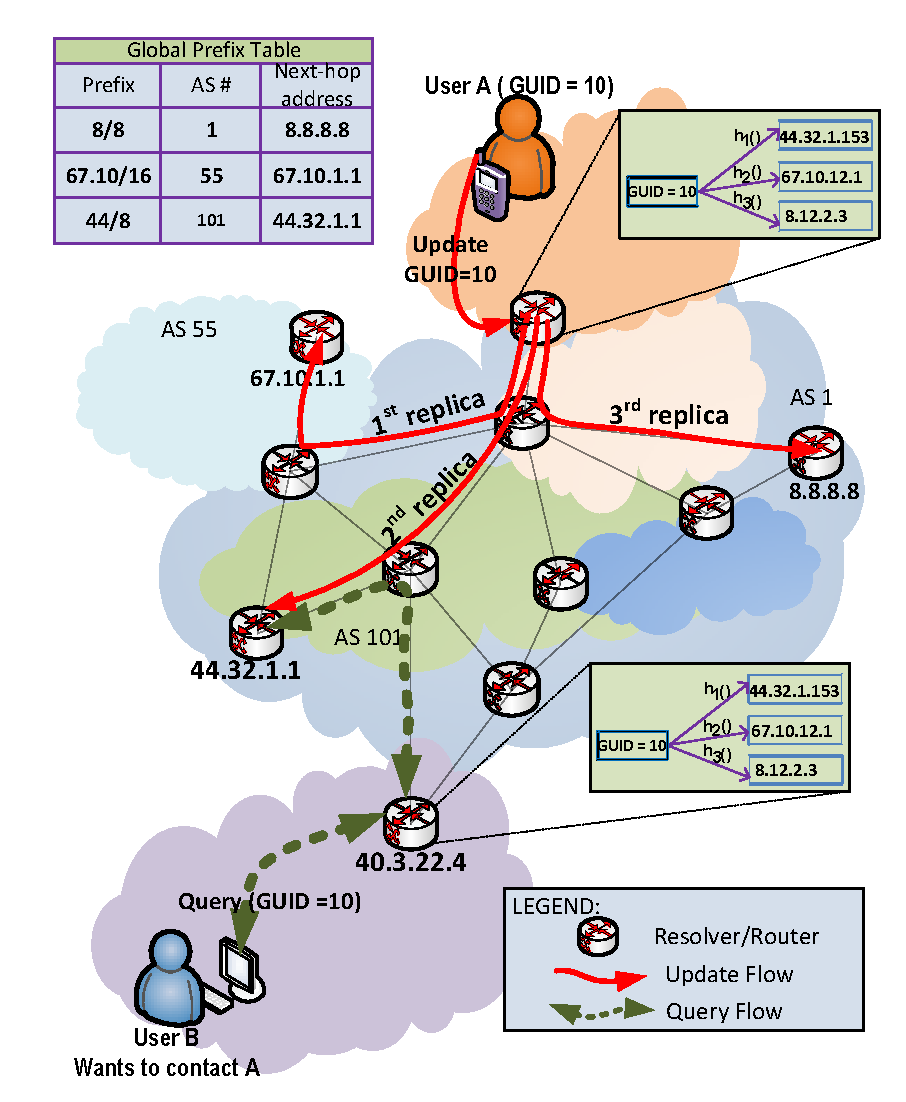
\includegraphics[width=0.4\textwidth]{figures/designV2.eps}
            \caption{DMap with K=3 independent hash functions}
            \label{fig:design}
            \vspace{-0.2in}
        \end{figure}
    \end{center}

\vspace{-0.2in}
Compared to other mapping schemes, one distinct feature of DMap is the direct participation of network routers in storing GUID$\rightarrow$NA mappings and in responding to updates and lookups. DMap does not require any additional state information as the IP reachability information is already made available by the BGP routing protocol.  In addition, we note that unlike many recent proposals~\cite{farinacci-alt,jen,jakab,mathy}, DMap does not distribute GUID mappings based on the assumption of the aggregate-ability of
the GUID space.  Our scheme is suitable for flat address spaces, which has been pointed out as a desirable feature for the Future Internet~\cite{andersen,moskowitz}.

\subsection{Handling Unallocated Network Addresses}
\label{subsec:ip_hole}

DMap hashes a GUID to an IP address, and stores the GUID mapping in the AS that announces this IP address.  Due to fragmentation in the IP address space, it is possible that the hashed IP address is not announced by any AS. This problem is referred to as the \emph{IP hole problem}. To understand the extent of this problem, we take a close look at today's IP address space. At present, 86\% of the $2^{32}$ IP addresses available in IPv4 are allocated to various entities~\cite{dix-ie}; the rest are reserved for other purposes including multicast, limited multicast, loopback address, broadcast, etc. Among the allocated addresses, 63.7\% of them are announced by one of the ASs. This leads to an overall 55\% announcement ratio over the entire IPv4 address space, which results in a 45\% chance that a randomly hashed $IP_x$ will belong to the set of unannounced addresses.
% or, IP holes.

 %While the technique produces the benefit of low latency naming look up and update since it only requires one overlay hop to reach the resolver, it suffers to the discontinuity of the address space. Since the hashed value of a GUID is equally distributed over address space, there is a probability that the hashed value falls into the address block that no organization have announced. We call the problem is \emph{IP hole effect}. % might need to change the name
%        For example, in current Internet, while there are $2^{32}$ possible IP addresses for IPv4, only 86\% of them are allocated to organizations. The rest are reserved for various purposes including multicast, limited multicast, loopback address, broadcast, etc. Among those allocated address, only 63.7\% of them are announced by organizations. As the result, the percentage of announced IP address is only 55\%[cite IP hole data] over the whole 32-bit IP space, giving the probability for a hashed result falling into one of the unannounced address is 45\%.

We address the IP hole problem by finding a deputy AS through rehashing if the IP address after the first hash falls into a hole. After $M-1$ rehashes, if the resulting address still falls into an IP hole, we pick the deputy AS as the one that announces the IP address that has the minimum \emph{IP distance} to the current hashed value. Given two k-bit addresses, A and B, their IP distance is defined as:
\begin{center}  %\vspace{-0.1in}
$IP\_distance_{[A,B]} = \displaystyle\sum\limits_{i=0}^{k-1} |A_i - B_i|*2^{i}.$ \end{center}
We further define the IP distance between an address and an address block as the minimum IP distance between that address to all addresses in the block. In this way, we can guarantee that a deputy AS can always be found.

There is a concern that the above method may introduce load imbalance among ASs: the AS that announces an IP address that is adjacent to a large set of reserved addresses (thus unannounced) may become a popular deputy AS and needs to store a large number of mappings. Fortunately, the probability of reaching an IP hole after $M$ hashes decreases rapidly with increasing $M$.
For instance, this probability is as low as 0.034\% for $M=10$. As a result, the chances that we need to resort to the ASs that announce the IP addresses with the minimum IP distances to the holes are very low.

Algorithm \ref{alg:rehashing} summarizes the steps taken by the border gateway to deal with the IP hole problem. Since hashing, rehashing and prefix matching processes are done locally by the border gateway, these operations introduce very little delay to the network.
       {
        \begin{algorithm}
            \small
            \SetAlFnt{\small\sf}
            \SetKwData{numbtry}{number\_of\_tries}
            \SetKwData{nearestPrefixID}{nearestPrefixID}
            \SetKwData{mindist}{min\_distance}
            \SetKwData{result}{result} %declare
            \SetKwFunction{lpm}{Longest\_Prefix\_Matching}
            \SetKwFunction{ipd}{IP\_distance}
            \SetKwFunction{findClosestPrefix}{find\_closest\_prefix} 
            \SetKwFunction{Hash}{hash}
            \SetKwInOut{Input}{input}
            \SetKwInOut{Output}{output}
            \Input{GUID - the $GUID$ to be hashed \\ \hspace{0.5cm}$M$ - maximum number of rehashing}
            \Output{An address guaranteed to be found in prefix table}
            \BlankLine
            $\numbtry \leftarrow 0 ;$\;
            $\result \leftarrow \Hash{GUID};$\;
            \While{ ($\numbtry < M $)}{
                \If{\lpm{\result} $>$ 0}{
                \Return \result; //ended here if found\;
                }
                 {// no prefix was found}\;
                $\result \leftarrow \Hash{\result}; $\;
                $\numbtry \leftarrow \numbtry+1 ;$\;
            }
            //No match found after M hashes\;            
	         \nearestPrefixID = findNearestPrefix(\result); 
%            $\mindist \leftarrow 2^{32}$;\;
%            \lForEach{prefix $i$ in the Prefix Table}{\;
%               \If{\ipd{\result,prefix $i$} $<$ \mindist}{
%                   \mindist $\leftarrow$ \ipd{\result to the prefix};\;
%                }
%            }
			\BlankLine
            \Return An address in \nearestPrefixID;
         \caption{Hashing GUID to address space} \label{alg:rehashing}
        \end{algorithm}\vspace{-12pt}
        }

When extending DMap to other network address schemes, such as IPv6, we need to rethink how we deal with the IP hole problem as these network address spaces may have substantially more holes than used address segments. To address such sparse address spaces, we propose to use a two-level indexing method to index each announced address segment: bucket ID and segment ID within that bucket. Suppose we have $N$ buckets, each with a capacity of $S$ segments. We make $N$ large so that $S$ can be kept small. Given a GUID, we run two hash functions, the first one mapping the GUID to bucket ID, and the other one mapping the GUID to the segment ID. Figure \ref{fig:bucketing} illustrates the bucketing scheme.

 \begin{center}
        %\vspace{-0.2in}
        \begin{figure}[t]
            \centering
            \includegraphics[width=0.5\textwidth]{figures/bucketting.eps}
            \caption{Bucketing scheme handling non-contiguous address space issue}
            \label{fig:bucketing}
            \vspace{-0.2in}
        \end{figure}
    \end{center}

%\subsection{Replication}
%\label{subsubsec:replication}
%To enhance DIHT's reliability and further reduce access latencies, we increase the number of resolvers responsible for each mapping entry by having the border gateways employ $K$ parallel hash functions at the time of update and query. During insertion or update, the border gateway applies Algorithm~\ref{alg:rehashing} $K$ times using independent hash functions on each iteration to obtain $K$ valid addresses. The mapping is stored in all the $K$ ASs responsible for the resulting addresses, thus creating storage replicas for each entry in the mapping table. To lookup a mapping entry, the gateway router selects the closest AS (in terms of path cost obtained from the BGP table) among the $K$ ASs that maintain the required mapping.
%After receiving the query, the border gateway applies Algorithm \ref{alg:rehashing} for K times with K different hashing functions to obtain K valid resolvers's addresses. Among these K resolver, It looks at the prefix table to choose the closest one. The notion of `closest' can be measure in terms of BGP distance (e.g. hop counts), or IP distance as mentioned in the previous subsection.
%This replicating technique leads to two important benefits - reduced lookup latencies and increased resilience to random failures. Firstly, with randomized replication, a gateway is more likely to find a nearby AS which stores the required mapping. We show in Section~\ref{sec:evaluation} that as $K$ increASs from 1 to 5, the 95th percentile lookup latency reduces from 202ms to 91ms. Secondly, as the number of replicas increASs, the resilience of the system is also greatly improved as the probability of two distant routers failing simultaneously is very low. Figure \ref{fig:design} illustrates an example of the update and query process with $K=3$. Finally, we note that this method interleaves the mapping replicas between ASs in contrast to exact replication of all the mappings from one AS to another, thus adding resilience random failures.

%The improvement in latency and reliability, however, comes with an increased storage requirement and enhanced complexity in the update process. A careful analysis based on the bounds on requirements and capabilities of the network is thus required to select an appropriate value for $K$.
        %Having too many replica can leads to increase in update delay and introduce addional network traffic. As the result, we need to carefully choose value for K in our design.
        %While it is obvious to see the query latency reduces as higher K is used, K can not be arbitrarily increased due to update propagation delay. Specifically, propagation delay for each update equals to the largest update delay to individual resolver, assuming the gateway simultaneously updates to all resolvers at once. Hence the inherent trade of between query latency and update latency must be taken into account when K is being used as the knob to tuning the network's performance

\vspace{-0.3in}
\subsection{Spatial Locality and Local Replication}
\label{sec:locality}

The main advantage of DMap lies in its simplicity: hashing a GUID to a random AS.  However, this random placement ignores locality, and so may degrade performance.  Having multiple replicas partially addresses this problem, but it still has the inherent problem of a direct hashing scheme: the GUID mappings are stored at faraway ASs when the host and requestor are close to each other.  Thus, we enhance the baseline DMap for an expected common case of when a requesting node is attached to the same AS as the GUID that it is resolving.  To leverage this \emph{spatial locality}, DMAP stores an additional replica of a GUID mapping at its attached AS.  When a host registers/updates its GUID, it creates/updates a local copy (at its attached AS) in addition to creating/updating the $K$ ``global'' copies. When a node needs to lookup a GUID, it sends out a local and a global lookup simultaneously.  When the host and the requester are from the same AS, the local request should lead to significantly reduced lookup latency.

% \begin{center}
%        \vspace{-0.2in}
%        \begin{figure}[t]
%            \centering
%            \includegraphics[width=0.5\textwidth]{figures/localCache.eps}
%            \caption{Local replication enhancement}
%            \label{fig:local_rep}
%            \vspace{-0.2in}
%        \end{figure}
%  \end{center}
\subsection{Inconsistent GUID$\rightarrow$NA Mappings}
\label{sub:inconsistency}

\subsubsection{BGP Churn} Since a change in the prefix announcements directly influences DMap, we analyze the potential effects of BGP churn. A long term study of BGP churn evolution~\cite{elmokashfi} shows that a major reason for churn in the BGP tables is router configuration mistakes or other anomalies. Changes in prefix announcements occur when an AS withdraws a previously announced prefix or announces a new prefix.  The actual rate of new prefix announcement and prefix withdrawal is small, with the former dominating the latter.

When an AS withdraws a certain prefix, all the mappings previously hosted by the AS whose GUIDs are hashed to the withdrawn IP addresses will become unaccessible, resulting in what we call \emph{orphan mappings}.   To address this problem, we let the withdrawing AS run the IP hole protocol to find a deputy AS for these mappings before withdrawing. It sends  a \emph{GUID insert messages} to the deputy AS and deletes its own copy of the mapping. Subsequent queries will then hit an IP hole. Following the same IP hole protocol, they will reach the deputy AS and find the mapping.

Announcing new prefixes can also result in orphan mappings. The GUIDs that were originally hashed to these IP addresses had followed the IP hole procedure to a ``deputy'' AS, and announcing these addresses now can make the mappings on the deputy AS orphan mappings. As a result, queries that reach the announcing AS will not find the mappings, while the mappings on the deputy AS become inaccessible. To solve this problem, when the announcing AS receives a query and finds the mapping missing, it sends a \emph{GUID migration message} to the deputy AS to relocate the mapping to itself. This operation could cause a negligible one-time overhead, which only occurs for the first query after the announcement.


%{\bf Need to mention Latency vs. BGP churn result here}

%In the latter case, where an AS announces new prefix, it becomes much more tricky. There will be queries that go to the AS with GUID that does not stored on any of the AS's border gateways, since it is stored in other AS that is behind the current AS in the hashing chain. In such cASs, the border gateway of the newly announced AS has to (1) first verify that he is on the hash chain of of that GUID, which can be done simply by applying K hash functions, m times for each on the given GUID. After positively confirmed, (2) the border gateway must go the the address right after him on the hashing chain to get the GUID and (3) inform that the mapping now becomes orphan to the AS right behind him so that the behind AS can start collecting garbage, certainly after a verification. The border gateway then stores the mapping on to permanent memory in order to be ready for the next query of the same GUID. Note that to reduce the user visibility on prefix change, the border gateway can in parallel issues P query to P resolvers, with $P<K$.

\subsubsection{Mobility} Mobility can also lead to inconsistencies in DMap. Suppose host $X$, with GUID $G_x$, is connected to AS $A$. As a result, DMap has the mapping $(G_x : A)$. Then suppose $X$ moves to AS $A'$ at time $t_0$, and its mapping will be updated to  $(G_x : A')$ at time $t_1$.  While we expect $t_1-t_0$ to be small, it is possible for a querying node to get the old mapping right after X has moved.  The querying node will then be unable to communicate with $X$.
In this case, the querying node should mark the mapping as obsolete, and 
keep checking until it receives an updated one.

\subsubsection{Router Failure} An AS can lose part or all of its mappings due to router failure. This is a rare event, but we need to address the resulting complication.  If a lookup request reaches an AS, but cannot find the mapping due to this problem, the requestor will wait for a timeout. Following the timeout, the requestor will contact the next mapping replica (remembering we have $K$ replicas in total). We note that the probability for $K$ Internet routes to fail at the same time is extremely low, and thus our replication strategy also improves system resilience and reliability.

\section{Evaluation}
\label{sec:evaluation}

In this section, we present the results from a detailed performance evaluation of the DMap scheme using a mix of qualitative reasoning and event-based simulation.

\subsection{Storage and Traffic Overhead}
To analyze the storage requirements in absence of specifications about the GUID/NA lengths and related headers, we make the following assumptions. We assume flat GUIDs of length 160 bits, each associated with a maximum of 5 NAs (accounting for multi-homed devices) of length 32 bits each. 32 bits of additional overhead per mapping entry is assumed which could include type of service, priority and other meta information. Each mapping entry thus has a size of 160 + 32x5 + 32 = 352 bits. We assume a total of 5 billion GUIDs, roughly equal to the present number of mobile devices, and a replication factor of $K = 5$. Based on the average prefix announcement by individual ASs as determined from a current snapshot of the BGP table~\cite{dix-ie}, the storage requirements per AS, assuming proportional distribution, is only 173 Mbits.  This storage requirement is quite modest, even if it is multiplied several times to include non-mobile devices as well as future growth.

The update traffic overhead is also a key parameter of interest in ensuring scalability. The DMap technique reduces the traffic overhead in comparison to other mapping schemes by: (a) Ensuring a single overlay-hop path to a storage location, (b) Not adding any table maintenance traffic as required in DHT schemes. Using a broad estimate of the 5 Billion GUIDs being those of mobile hosts which update their GUID$\rightarrow$NA mapping at an average rate of 100 updates/day, the world-wide combined update traffic would be $\sim$10 Gb/s, a minute fraction of the overall Internet traffic of $\sim 50$x$10^6$ Gb/s as of 2010~\cite{cisco-2010}.

\subsection{Query Response Time and Load}
%Next we describe our event-based simulation setup and present results which characterize the critical parameters of query latency and load distribution.
The round trip response time of a query is composed of: (i) $K$ longest prefix matchings at the local gateway router, (ii) network latency between the query source and the chosen destination AS, (iii) the queuing and processing delay of the mapping server at the destination AS and (iv) the return network latency between the destination AS and the query source. Since routers use fast longest prefix match algorithms, requiring on order of 100 instructions per lookup, i.e. $\sim$30 nanoseconds on a 3 GHz processor~\cite{Degermark:1997}, we ignore this component in our evaluation. Also sufficient resources are assumed at the mapping server to make the queueing and processing delay very small compared to the round trip latency. Note that this process does not add any delays to the normal data packets as the steps described above are only applied to GUID query packets and are assumed to be handled at a separate compute layer at the gateway router.

%As described in Section~\ref{sec:design}, a GUID query process involves the following steps: (i) the query is forwarded from the host to its gateway router, (ii) the gateway router hashes the GUID and uses longest prefix matching searches on its local copy of the BGP table to ensure the hashed IP is announced by an AS; rehashing is done if required, (iii) the query is directed to the closest of the $K$ mapping servers - assumption about the closeness metric is described below, (iv)

\subsubsection{Simulation and Workloads}
%\subsubsection{Event-based Simulator Architecture}
%\label{subsec:evaluation_setup}

We develop a discrete-event simulator consisting of $\sim$26000 nodes, each emulating an AS. The connectivity graph of the network, inter-AS and intra-AS connectivity latencies, and the announced IP prefix list are derived from measurement driven data as described below. We consider three types of events:  GUID inserts, GUID updates and GUID lookups.% are pre-generated and organized into a global queue.  The global queue guarantees that the order of events on each run are the same and will lead to the same outcome. The event controller processes events in the global queue in sequential order following the sequence of operations outlined in~\ref{sec:design} to process each kind of event. For each query event, the total latency is computed and stored as a data point. The simulation concludes with data gathering from each AS in terms of number of GUIDs stored and average query/update rates.
\footnote{The source code for our simulator is available at \cite{sourceCode_NRS}}

%\subsubsection{Data Sources}
%\label{subsubsec:dataSources}
We use the AS-level topology of the current Internet as our network model by extracting the following real-measurement data from the DIMES database~\cite{shavitt}: (i) Connectivity graph containing 26,424 ASs and 90,267 direct links between them, (ii) Average end-to-end latencies between each pair of AS and within each AS. The DIMES database provides end-to-end median latency for about 9 million pairs of hosts which are either within the same AS or in different ASs. From this dataset, we extract the average inter-AS and intra-AS latency since we only work with an AS-level network topology in our simulation. Due to the inherent incompleteness of real-trace data, intra-AS latency numbers are not available for about 6\% of the ASs that are involved in the storage or transit of the mapping data. For these ASs, we use the median value (3.5 ms) of the set of available intra-AS latencies as a working solution. %We note that there are other measurement driven sources for AS topology data, for example~\cite{madhyastha} and~\cite{claffy}, but we found DIMES to have a more complete view of the AS-level graph compared to any other database.
%\textbf{We assume that the network delay component of the total query response time dominates processing and queueing delays at the server where the queries are resolved.}
%For route selection, we use minimum latency paths between each pair of source and destination AS. %and make a conscious decision of not employing one of many path inference schemes such as~\cite{gao,weinsberg} that aim at also incorporating estimated policies at each AS. The dynamic nature of AS relationships, multi-homed networks and hidden/misconfigured policies prevalent in the Internet limits the accuracy of such schemes, introducing an uncharacterizable source of error in the results. We chose to present our results with the caveat of AS policy ignorance instead of adding unknown inference errors.

Since our scheme allocates GUIDs to ASs according to the prefix announcements, we use a complete list of IP prefixes advertised in the Internet default free zone (DFZ), as seen by APNIC's router at DIX-IE in Tokyo, Japan~\cite{dix-ie}. This dataset consists of roughly 330,000 prefixes spanning close to 52\% of the 32 bit IP address space which is consistent with recent estimates~\cite{elmokashfi} about the size of the prefix tables in DFZ routers. We confirm our results with two other prefix tables taken from BGP routers in the continental USA and Europe respectively and observe similar trends.


To discard any location bias and to incorporate the global scale of operation, we use another dataset from DIMES that contains the number of end-nodes connected to ASs 
to characterize the distribution of the source of GUID insert and query. Each GUID in our simulation originates from a randomly picked source AS, where the probability of choosing a certain AS is weighted in proportion to the number of end-nodes found in that AS.
%The end-result emulates a real deployment scenario in which more populated areas (characterized by high number of IP end-nodes) will generate more GUID queries compared to less populated areas. We note that the nature of trace collection employed by DIMES might introduce a bias due to non-uniformity of vantage point distribution (though shown to be small), however we do not take this into account in our simulation.

%\subsubsection{Popularity Model}

The number of queries for any GUID depends on its popularity amongst Internet hosts. In order to capture the effects of the wide variations in host popularity, %we use a parametric model for generating the query events in our simulation.
%
%Large scale measurement studies of web, peer-to-peer and content popularity in the Internet have been shown to closely
we use a Mandelbrot-Zipf distribution~\cite{krashakov, Saleh-06} to model the varying host popularity. The Mandelbrot-Zipf distribution defines the probability of accessing an object at rank k out of N available objects as:
\begin{equation}    
p(k) = \frac{H}{(k+q)^\alpha},
\end{equation}
where $H = 1/\sum_{k=1}^N 1/(k+q)^\alpha$, with $\alpha$ determining the skewness and $q$ affecting the ``flatness'' of the peak. We use a value of $\alpha = 1.02, q = 100$ following the arguments in~\cite{Saleh-06}.

\begin{center}
	\begin{figure}[t]
	%\vspace{-0.2in}
	\centering
	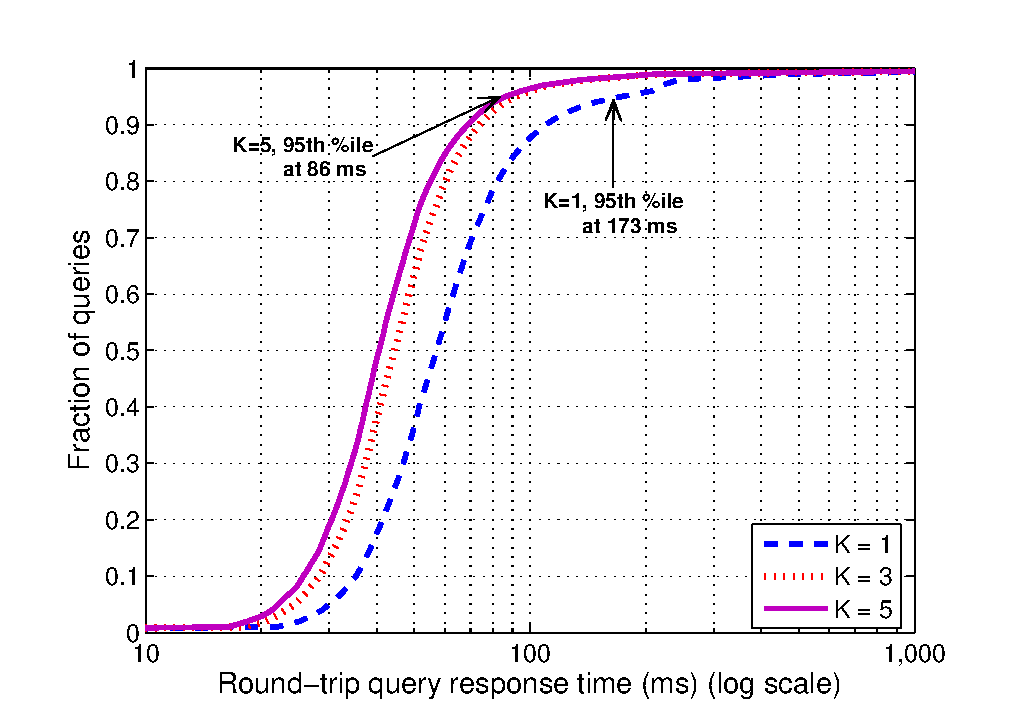
\includegraphics[width=0.4\textwidth]{figures/queryLatency}
	\caption{Round trip query response times}
	\label{fig:queryLatency}
	\vspace{-0.15in}
	\end{figure}
\end{center}

\vspace{-0.3in}

\subsubsection{Results}
We present two sets of results that characterize the query response time and the load distribution of our scheme respectively.

\paragraph{Query Response Time} We evaluate the query response time for DMap
by inserting $10^5$ GUIDs and generating $10^6$ queries according to the popularity model. By repeated trials with increasing number of GUIDs/queries, we
verified that the response times converged after reaching the above configuration and larger numbers are not necessary. When we store a mapping at multiple locations, i.e., $K>1$, in the results below, we assume that the querying node has sufficient information to choose the location with the lowest response time. We note that in today's Internet, this information is only partially available, but at the least, each AS has hop count information for reaching
all other ASs through the routing protocol. Using least
hop count instead of lowest response time leads to similar results
albeit with marginally increased latencies. We would also emphasize that many techniques are being proposed to better estimate the response times~\cite{Godfrey2009}.

 %(for example, median latency changes from
%40ms to 50ms for the $K=5$ curve in Figure~\ref{fig:queryLatency})


%{\bf Thu: need to
%work in a few words about what happens if we use hop counts
%  instead.}

Figure~\ref{fig:queryLatency} plots the
cumulative distribution function (CDF) of the round trip query
response times with varying $K$ values. We make two observations. First, with $K=5$, 95\% of the queries complete within 86ms. This is well within the range needed for voice
call handoffs~\cite{3gpp}. Indeed, given that many WiFi and IP handoff protocols are often on the order of 0.5-1 second~\cite{vassiliou_2009,Mishra:2003:EAI:956981.956990},
DMap updates would not introduce an undue additional burden. Second, storing each GUID mapping in multiple locations can significantly reduce query response
times, as it allows a querying node to choose the replica that is
``closest'' to itself, thus addressing the locality of the requests. The effect of increasing $K$ can be clearly seen with the leftward shift of the CDF curve as we increase the value
of $K$. In particular, the mean, median and $95^{th}$ percentile query
latencies of $K = 1$ and $K = 5$ cases are tabulated in
Table~\ref{table:latency}, which shows a marked decrease in the tail of the response time distribution.

However, even the curve for $K=5$ has a relatively long tail.  This long tail arises from a few queries originating from those ASs with unusually long intra-AS response times, according to the DIMES dataset. For example, the 18 queries with the longest response times all originated from AS 23951, a small AS registered in Indonesia with a one-way latency of more than 2.3 seconds on each of its outgoing links.
\begin{table}[b]
\vspace{-0.1in}
\centering
\begin{tabular}{|c|c|c|c|}
\hline
\multicolumn{1}{|c|}{{\bf {\em K}}} & \multicolumn{3}{|c|}{{\bf Round Trip
    Query Response Time (ms)}}\\
\cline{2-4}
 & {\bf Mean} & {\bf Median} & {\bf 95th percentile}\\
\hline
1 & 74.5 & 57.1 & 172.8\\
\hline
5 & 49.1 & 40.5 & 86.1\\
\hline
\end{tabular}
\caption{Query Response Time Statistics for $K $ = 1, 5}
\label{table:latency}
\end{table}

\begin{center}
\begin{figure}[t]
\vspace{-0.2in}
\centering
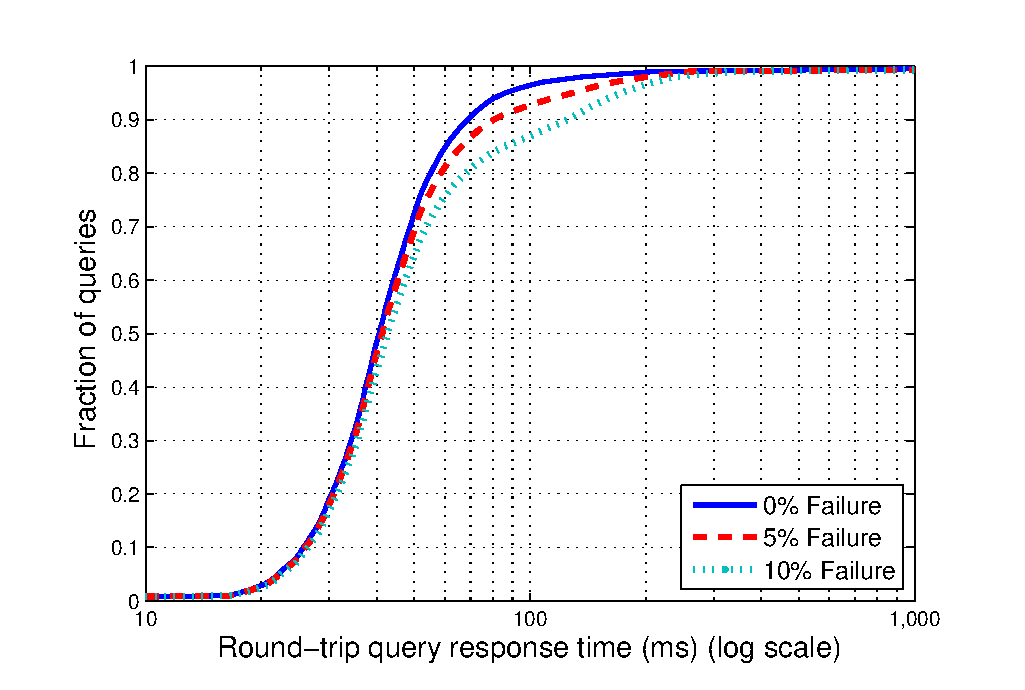
\includegraphics[width=0.4\textwidth]{figures/queryLatencyVsChurn}
\caption{Effect of BGP Churn on query response times.}
\label{fig:queryLatency-BGP-churn}
\vspace{-0.2in}
\end{figure}
\end{center}

\vspace{-0.3in}

\paragraph{Impact of BGP Churn}  %{\bf (Thu: this is very rough.  It
  %would be nice if Rich or Yanyong or someone who understands BGP
 % better than I can help improve this paragraph a little bit.}
The above study assumes that the BGP table at the query origin exactly
reflects the current state of the Internet. However, BGP tables at
different places in the Internet can be inconsistent because of new prefix announcements or prefix withdrawals. This inconsistency may have an adverse impact on the overall query response times as the query may reach an AS which does not host the requested mapping. In this situation, the AS will then reply with a ``GUID missing'' message, and the querying node will have to contact another replica.  %{\bf Thu: Can this
%  lead to another failure?}
Thus, a query may require multiple round-trips to different ASs for each resolution.
We note that the probability of two churns occurring at the same time for the same GUID is negligible.
  %Since our hashing scheme only depends on the information on
%the source AS for IP prefixes, we only need to consider BGP updates
%that result in origin AS changes for any IP prefix.
%
%In~\cite{qiu-2006}, the authors observe that ``origin changes account
%for less than 2\% of the BGP update traffic with more than 90\% of the
%prefixes being consistently originated by the same AS for an entire
%year. For those prefixes involved in origin changes, approximately 57\% have only one change across the year, implying that these changes are indeed permanent.'' In~\cite{mahajan-NANOG23}, Mahajan et al. observe that ``more than 2\% of the prefixes experience an origin change during the day.''
Here, we conduct a set of experiments to quantify the impact of this inconsistency caused by BGP churn. In the experiments, we vary the percentage of prefixes that are newly announced or withdrawn from 0 to 10\%. Figure~\ref{fig:queryLatency-BGP-churn} plots the CDF of the query
response times for $K=5$ and 0\% to 10\% lookup failures.  A 5\%
failure rate, which already seems pessimistic according
to~\cite{qiu-2006,mahajan-NANOG23}, shifts the median and 95th
percentile from 40.5ms and 86.1ms to 41.3ms and 129.1ms,
respectively.  %{\bf Thu: Akash, Tam, in the powerpoint, you have
 % numbers of 20\% failure rate.  But, I think that this is too
 % pessimistic.  I prefer using the 5\% numbers unless you think that
 % this is wrong.} \textbf{Akash: Sure, I entered the values}

\vspace{0.1in} \paragraph{Storage Distribution}
We next study the distribution of GUID$\rightarrow$NA mappings amongst ASs to evaluate
DMap's ability to spread the storage load proportional to the size of
the ASs. We measure storage load using the {\em Normalized Load
  Ratio} (NLR) at each AS, which is defined as the ratio of the
percentage of GUIDs assigned to an AS divided by the percentage of IP
addresses advertised by that AS. For example if an AS announces a $/8$
prefix, corresponding to 0.39\% of the 32 bit IP space and is assigned
20,000 out of a total of 1 Million GUIDs, i.e., 2\% of GUIDs, then its
normalized load would be 2/0.39 $\simeq$ 5. Ideally, each AS's NLR
would be 1.

Figure~\ref{fig:loadDistr} plots the CDF of the NLR when we inserted
from $10^5$ to $10^7$ GUIDs, with $K=5$.
%(In this experiment, $K>1$ simply equals inserting more GUIDs so we only discuss results for $K=1$.)
We observe that for $10^7$ GUIDs, %88\% of the ASs had NLRs between
%0.5 and 1.5 {\bf Can change the 0.5 to 1.5 a little bit to get a
%  ``nicer'' percentage if desired}. \textbf{Akash: Maybe,
93\% of the ASes had NLRs between 0.4 and 1.6. Further, we observe that as the
number of GUIDs increases from $10^5$ to $10^7$, the CDF becomes much
sharper around NLR equal to 1 (with a shorter tail). This suggests that DMap can distribute the storage load better when the system scales.
%distribution of
%storage load improves with the number of GUIDs in the system.
These results show that DMap does a %extremely
very good job of spreading out the
storage load proportional to the percentage of the IP space that an AS
claims.

Interestingly, the median NLR value is 1.16. The fact that the median NLR value is greater than 1 is expected since in addition to its fair share of GUIDs, many ASs are also allocated a portion of the GUIDs that has hashed values after M retries falling in the IP holes as described in Section~\ref{subsec:ip_hole}.

%we have also studied the tail of the CDF for $10^7$ GUIDs in
%Figure~\ref{fig:loadDistr}. There were only 16 ASs with NLR greater
%than 3. None of these ASs received additional load because of IP
%holes. %{\bf Thu: Akash, Tam, please check this if you can. If you can
  %only check a subset, let me know.} \textbf{Akash: Checked all; none of the 16
  %announces addresses which are adjacent to a hole.} All of these are small ASes,
%i.e., advertising 256--2304 addresses, that received several extra
%GUIDs.  We believe that such slight overloading is not a problem, and
%will further reduce as the number of GUIDs increase.
\iffalse
	\begin{table}[b]
	\centering
	\begin{tabular}{|c|c|c|c|}
	\hline
	\% Local & Mean & Median & 95th Percentile\\
	Queries & Response Time & Response Time & Response Time\\
	\hline
	0 & 49.1 & 40.5 & 86.1\\
	\hline
	10 & 45.9 & 38.6 & 84.1\\
	\hline
	20 & 43.2 & 36.8 & 82.2\\
	\hline
	30 & 40.4 & 34.6 & 80.2\\
	\hline
	\end{tabular}
	\caption{Round trip response time (ms) for varying spatial locality ($K =5$)}
	\label{table:locality}
	\end{table}
\fi
%Modeling host mobility in the Internet has been the focus of a large number of studies, though most models aim to characterize specific wireless environments, for example, cellular networks~\cite{Hyytia-07}, vehicular networks~\cite{Harri-06} and ad-hoc networks~\cite{Lin-04}. Since our focus is not on modeling the movement of hosts but to capture the GUID-to-NA mapping update they might produce, we abstract out a simple discrete model for the number of mapping updates for each GUID. In this model, GUIDs are classified into four broad classes: fast mobility, medium mobility, low mobility and static. Inter-update times in each of the three mobile classes are distributed exponentially with a different mean value per class. The proportion of fixed and mobile hosts is kept as a parameter $\beta$, while the probability of a mobile host belonging to each of the three mobile classes being kept equal. In order to include the reality of most popular hosts being static, we include a parametric threshold $\tau$, which defines the popularity level above which all hosts are static. Figures ? and ? shows the popularity and mobility models used in our simulation.

%It then produces a inter-domain routing table for all ASs in the network. We consider that each AS has one participating BGP router.
\iffalse
	\begin{center}
	\begin{figure}[t]
	%\vspace{-0.2in}
	\centering
	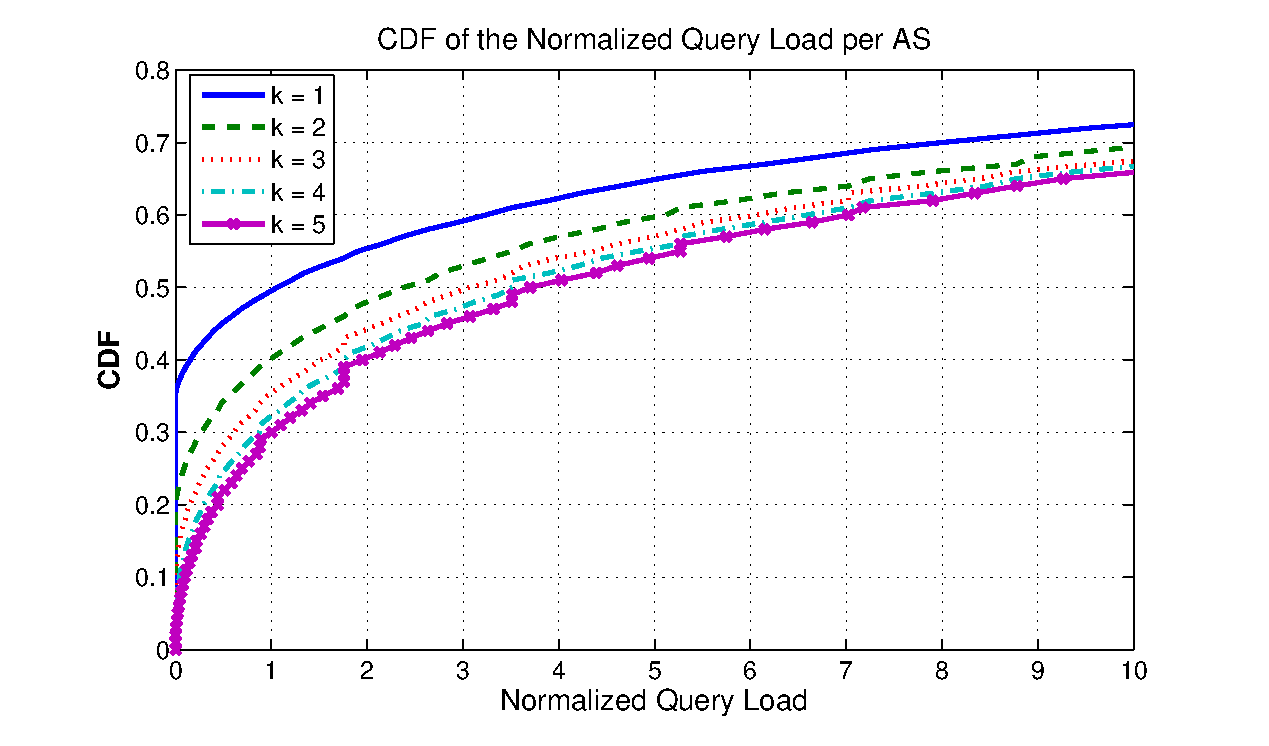
\includegraphics[width=0.5\textwidth]{figures/queryLoadVsK1}
	\caption{Empirical CDF of the Normalized Query Load}
	\label{fig:queryLatency}
	%\vspace{-0.2in}
	\end{figure}
	\end{center}
	
	\begin{center}
	\begin{figure}[t]
	%\vspace{-0.2in}
	\centering
	\includegraphics[width=0.5\textwidth]{figures/storageLoadK-5}
	\caption{Empirical CDF of the Normalized Storage Load}
	\label{fig:queryLatency}
	%\vspace{-0.2in}
	\end{figure}
	\end{center}
	
	\begin{center}
	\begin{figure}[t]
	%\vspace{-0.2in}
	\centering
	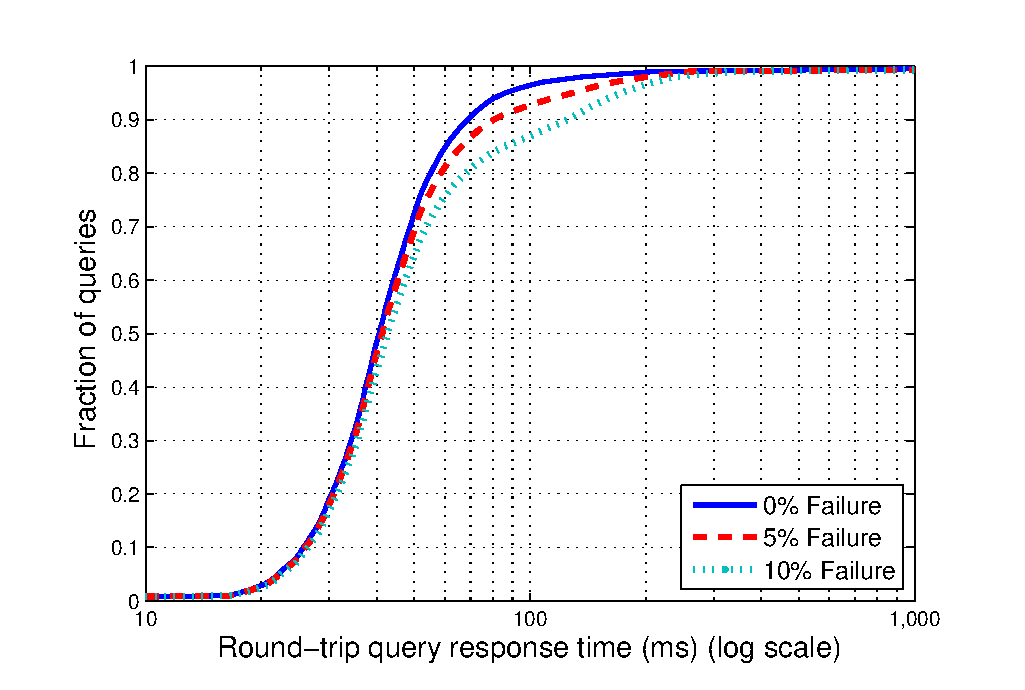
\includegraphics[width=0.5\textwidth]{figures/queryLatencyVsChurn}
	\caption{Effect of BGP Churn on query latency}
	\label{fig:queryLatency}
	%\vspace{-0.2in}
	\end{figure}
	\end{center}
\fi
%\subsection{Future Internet model}

%TBA

%Jun's estimation goes here


%This section present our large scale simulation implementation.

%Our simulation takes description of the network topology at layer-3 from netDimes \cite{} including 90 thousands single-hop AS-to-AS connection, from which we build the connectivity graph between ASes. We derives from 9 Millions  end-to-end traces from netDimes to have an estimation of intra-AS latency for every AS. Let $L_{AS1}$ and $L_{AS2}$ are intra AS latency of AS1 and AS2 accordingly.  If there is a connectivity from AS1 to AS2, the latency for every single-hop AS-to-AS connection is compute as follow.

%We takes a list of IP prefixes from \cite{}, a Japanese BGP border gateway. it produces a inter-domain routing table for all routers in the network. That route selection process computes the shortest path according to  from the provided topology. One might argues that the route selection should follow BGP which also takes ASes' policies into account. However,  for simplicity, all policies should be reflected on the provided topology in our model, e.g. if an AS prefers one path over another, that preference should be represented in path's cost. Note that edges are directional.

%Once the topology is loaded, and the inter-domain routes have been computed, the Actuator starts processing events in global queue in sequential order. The global queue guarantees that the orders of events on each run are the same and will lead to the same outcome. That is in contrast with traditional discrete event where outcome depends on the seed of the pseudo random number generator. There are several types of events, including  GUID insert, GUID update, GUID lookup and BGP table update.

%For each insertion event extracted from the global even queue, Actuator applies k hash function on to that GUID, may rehash up to m times to get the hashed value felt into announced IP address, called IPx. For each IPx, Actuator lookup on AS prefix table to find the corresponding AS and destination IP address of BGP speaker's of that AS. It then get the list of  ASes that the request must be directed through in order to be delivered to that destination AS. For each AS on the path, Actuator updates the message counter of that AS, adjust the time stamp on that AS, and increase the time stamp for that request based on the latency of the passed through link. For timestamp adjustment on particular AS, Actuator assign the greater timestamp among <AS time stamp, message time stamp>  as the new time stamp for that AS. The message is forwarded on a AS-by-AS basis until it reaches its final destination. Upon delivered to the destination, destination AS update its GUID list with the new one, followed by GUID's time stamp.

%The actuator continues the simulation by popping the first event from the global queue, simulating the behavior at each router along the path. If the event is GIUD lookup or GIUP date, the steps tobe executed by the actuator are very much similar to that with aforementioned GUID insert.  If the event is BGP table update, the actuator takes the diff operation to compare the old table with the new one. It then identifies ASes that got affected from the change�


%We evaluate the DMap architecture using three different views of the structure of the Internet:

%(TBA:Change the three names)

%\begin{enumerate}
%\item Present day Internet: As a first step, we evaluate the performance of DMap over the Internet as it is today using measurement based model comprised of $\sim$17,000 ASs and $\sim$190,000 Points of Presence (PoPs). The connectivity graph between PoPs, link latencies and path prediction is derived from the iPlane project~\cite{IplaneNano09}, which provides a structural view of the Internet using measurements from distributed vantage points in the network.

%\item Removing the effects of path inefficiencies: To isolate the effects of path inefficiencies in the Internet from the irreducible path characteristics, we re-evaluate the performance numbers assuming a shortest path routing between ASs. The results show that a major portion of network delays are an artifact of path inefficiencies in the Internet which can be alleviated by routing improvements in the future Internet.
%
%\item Future Internet model: Finally, we define a simplistic, but pragmatic model of the future Internet topology and discuss the deployment and performance of the proposed DMap architecture in this context.
%
%\end{enumerate}
%%In this section, we present results from a large-scale event-based simulation study aimed at characterizing the performance of DMap. Our evaluation focuses on the following performance measures:

%%\subsection{Present day Internet}
%%
%In this section, we present results from a large-scale measurement driven, event-based simulation study aimed at characterizing the performance of DMap. Our evaluation focuses on the following performance measures:
%
%\begin{itemize}
%\item Query and Update Latency (Fig. ? \& Fig. ?)
%\item Storage Load Distribution ( )
%\item Query and Update Load Distribution ( )
%\item Probability of Retrieving Stale Mappings ( )
%\end{itemize}
%
%
%\subsubsection{Simulation setup}
%\label{subsec:evaluation_setup}
%
%%\subsubsection{Event-based Simulator Architecture}
%
%The discrete-event simulator consists of a measurement driven Internet topology model with $\sim$17,000 ASs encompassing $\sim$190,000 Points of Presence (PoPs). The connectivity graph between PoPs, link latencies and path prediction is derived from the iPlane project~\cite{IplaneNano09}, which provides a structural view of the Internet using measurements from distributed vantage points in the network. Two types of events: GUID updates and GUID queries are generated according to parametric popularity and mobility models, as described in Sec. ?. Each event is associated with a 3-tuple of \emph{ $<$ GUID $|$ Timestamp $|$ Source of query/update$>$}. The event list is pre-generated and organized into a global queue which guarantees that the order of events on each run are the same and will lead to the same outcome. The event controller processes events in the global queue in sequential order following the sequence of operations outlined in Section~\ref{sec:design} to process each kind of event. Data gathering is done per-event for end-to-end latency, staleness and per-AS for number of GUIDs stored, queries and updates received\footnote{The source code for our simulation is made available at \cite{sourceCode_NRS}}.

\begin{center}
\begin{figure}[t] 
\vspace{-0.2in}
\centering
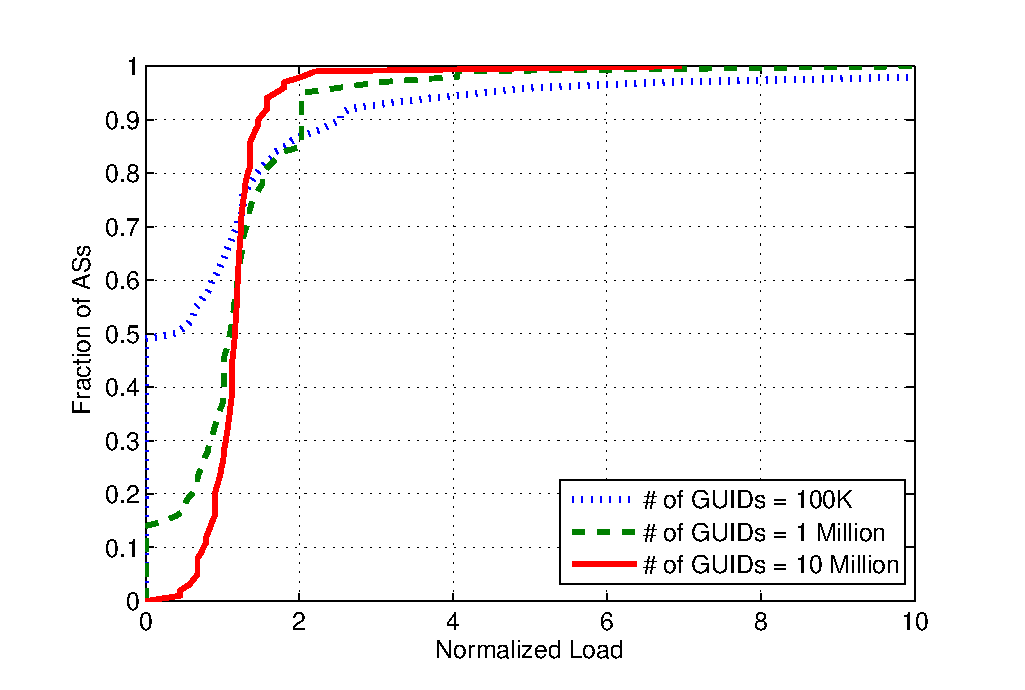
\includegraphics[width=0.4\textwidth]{figures/loadDistr}
\caption{Normalized Load Ratio per AS}
\label{fig:loadDistr}
\vspace{-0.2in}
\end{figure}
\end{center}
\vspace{-0.2in}




%%% Local Variables:
%%% mode: latex
%%% TeX-master: "paper"
%%% End:

\section{Analytical Model for Query Response Time}
\label{sec:model}
In this section we present an analytical model for an upper bound on the query response time and parametrically study its dependence on the Internet topology and replication factor $K$. While the simulation framework of Section \ref{sec:evaluation} shows the response time performance of DMap based on the current Internet topology, this analytical model allows us to estimate its performance based on a predicted future Internet model.
\subsection{The Jellyfish Model}
An accurate parametric model of the Internet topology is known to be a difficult endeavor due to the inherent complexities in routing policies, detour paths and limited visibility of the intra-AS structure~\cite{HeSF09}. The Jellyfish model, however, has been found to closely follow the evolution of the Internet topology at a relatively coarse scale~\cite{tauro-jellyfish}. In this paper, we build a Jellyfish model based on the PoP-level Internet topology. We first label the node with the highest degree as the root $v_0$ and the maximal clique\footnote[1]{clique: a completely connected subgraph of $G$.} containing $v_0$ as the {\em core}, denoted as $Shell\textrm{-}0$. Let $v$ be a non-root node and $j$ a non-negative integer. The smallest path length\footnote[2]{path length: the number of edges in the path, $i.e.$, that of the involved PoPs in the path minus 1.} from $v$ to a node in the core is its {\em distance to the core}. We use $Shell\textrm{-}j$ to denote the set of nodes whose degree is more than 1 (intermediate nodes) and whose distance to the core is $j$. We use $Hang\textrm{-}j$ to denote the set of nodes whose degree is 1 (leaf nodes) and whose distance to the core is $j+1$. These are standard notations in the Jellyfish model~\cite{HeSF09}. Then we have
\[
Layer(j) = Shell\textrm{-}j \cup Hang\textrm{-}(j-1) \textrm{~~for~}j \ge 1,
\]
and $Layer(0)=Shell \textrm{-} 0$. We further denote the total number of layers in the Internet PoP topology as $N$ and the percentage of nodes in layer $j$ by $r_j$; if $n$ is the total number of nodes in $G$, then $r_j = \left| Layer(j) \right| / n$. The separation of one degree nodes at each layer distinguishes between stub connections and transit connections which makes the model much closer to the Internet topology than a standard tree structure.

\subsection{Upper Bound for Query Response Times}
Following the above model, if we assume no peer links between the nodes inside each layer, then the distance between any two nodes $s$ and $t$ (in layers $j_s$ and $j_t$ respectively), $d(s, t)$,  is at most $j_s + j_t + 1$. Note that since the core forms a completely connected graph, all hops in the core are of length one.  To drive a simple parametric upper bound for the query response time, we assume that the network address space is uniformly distributed among the PoPs and all addresses within a PoP behave in an identical fashion. Following the algorithm described in Section \ref{sec:design}, let the source of a GUID query belong to PoP $s$ and let $t_1, t_2, \ldots, t_K$ be the destination PoPs for the query determined by the $K$ hash functions $h_1, h_2, \ldots, h_K$ applied on the GUID $G$. Assuming a linear relationship between PoP path length and response time, the query response time $\tau(s, G)$, is thus given by

\begin{equation}
\tau(s, G) = c_0 \cdot \min_{1 \le i \le K} d (s, t_i) + c_1,
\label{eq:tau}
\end{equation}
where $c_0$ and $c_1$ are constants. In order to average over all possible source and destination PoPs, we treat $d(s, t_i)$ as a random variable and find its probability distribution based on the $r_j$ values defined in the previous subsection. In the analysis, we use the standard notations $Pr (\cdot )$ and $Pr ( \cdot ~|~ \cdot )$ for the probability and conditional probability of argument events, and $ \mathbb{E}( \cdot )$ for the expected value of a random variable.

Given a uniformly selected source PoP, we have $Pr(s \in Layer(j) )= r_j$. Note that since DMap actually chooses a network address uniformly over all possible addresses, the $j^{th}$ layer could include a different number of addresses than the ratio $r_j$. Our analysis assumes the uniform distribution of addresses among PoPs but the model can be easily extended to non-uniform distributions by considering weights $w_s$ proportional to the number of addresses in PoP $s$. Since accurate estimates of such a distribution is not directly available through any of the Internet measurement frameworks, we assume $w_s = 1$ for all $s$. Based on the same assumptions, we have $Pr ( t_i  \in Layer (j_i) ) = r_{j_i}$ for each $i=1, 2, \ldots , K$ and $j_i=0, 1, 2, 3, 4, \ldots, N-1$. Thus the conditional probability of $d ( s, t_i ) \ge l+1$ given that $s \in Layer(j)$ is at most the percentage of nodes in $Layer(l-j) \cup Layer(l+1 - j ) \cdots \cup Layer(N-1) $. (Since $s$ is in $Layer(j)$, $d ( s, t_i ) = l+1$ when $t_i$ is in $Layer(l-j)$, $d ( s, t_i ) = l+2$ when $t_i$ is in $Layer(l+1-j)$ and so on in the worst case). In other words,
\begin{equation}
\begin{aligned}
& Pr\left(d (s, t_i) > l  ~\big|~ s \in Layer(j) \right)  \le  p_{j,l},
\\ \textrm{where }
& p_{j, l} \stackrel{def}{=} r_{l-j} + r_{l+1 - j} + r_{l+2 - j}\cdots
\\ \Rightarrow & \nonumber
Pr \left(  \min_{1 \le i \le K} d ( s, t_i ) > l  ~\big|~ s \in Layer(j)  \right)  \le  p_{j,l}^K,
\\ \Rightarrow & \nonumber
Pr \left(  \min_{1 \le i \le K} d ( s, t_i ) \le l  ~\big|~ s \in Layer(j)  \right)  >  1 - p_{j,l}^K,
\\ \Rightarrow & \label{CDF}
Pr \left(  \min_{1 \le i \le K} d ( s, t_i ) \le  l  \right)  >
\sum_{j=0}^{N-1} r_j ( 1 - p_{j,l}^K ).
\end{aligned}
\end{equation}

This provides an upper bound for the CDF of average distance from the source to the closest destination. Thus the probability that $\min_{1 \le i \le K} d ( s, t_i ) > l$ is at most $ 1 - q_l$, where we define $q_l$ as:
\[
q_{l} \stackrel{def}{=}\sum_{j=0}^{N-1} r_j \left( 1 - p_{j,l}^K \right),
\]
Finally, noting that the diameter of our PoP graph is $(N-1)+(N-1)+1 = 2N-1$ or less,
\begin{equation}
\begin{aligned}
 & \mathbb{E}\left( \min_{1 \le i \le K} d ( s, t_i ) \right) < \sum_{l=1}^{2N-1} (1-q_l)\\
 & \Rightarrow \mathbb{E} \left(\tau(s,G)\right) < c_0 \left(\sum_{l=1}^{2N-1} (1-q_l)\right) + c_1.
\end{aligned}
\end{equation}

\subsection{Analytical Results}

 We use the formulation derived above to study the response time upper bound in three different scenarios with varying number of replicas $K$. The first scenario reflects the current Internet topology, for which we use measured data from the iPlane project~\cite{madhyastha} for setting the parameters $r_j, j = 1,2,\ldots, N$. The data set shows a graph of 193,376 nodes within 8 layers and more than 60\% of the nodes residing in layers 3 and 4. The next two scenarios model the medium-term and long-term future Internet topologies. In order to come up with models for the future Internet, we leverage the following two distinct trends observed from the widely regarded CAIDA measurement framework~\cite{caida-main}: (i) The number of nodes are growing almost linearly with time, (ii) The topology graph is getting flatter with time, i.e. ASs are obtaining more direct paths to the core. Extrapolating these trends, we model the medium-term (5-10 years) future Internet as having 20\% more nodes than present contained in 6 layers. Similarly, the long-term (25-30 years) future Internet model contains double the number of nodes contained in 4 layers. Figure~\ref{fig:resAnalysis} shows the analytical upper bound of average query response time for the three scenarios using the measured least squared error values for ${c_0,c_1} = {10.6,8.3}$. The plot shows that based on the predicted future Internet topology, response time upper bounds for DMap queries become smaller with the evolution. Also, the analysis clearly indicates that increasing the replica number results in diminishing returns beyond a few replicas. We note that actual values for the query response upper bound will typically be smaller than the ones obtained in this analysis, since we did not consider the presence of peering links between nodes in the same layer.\vspace{-0.15in}
\begin{center}
\begin{figure}[t]
\vspace{-0.2in}
\centering
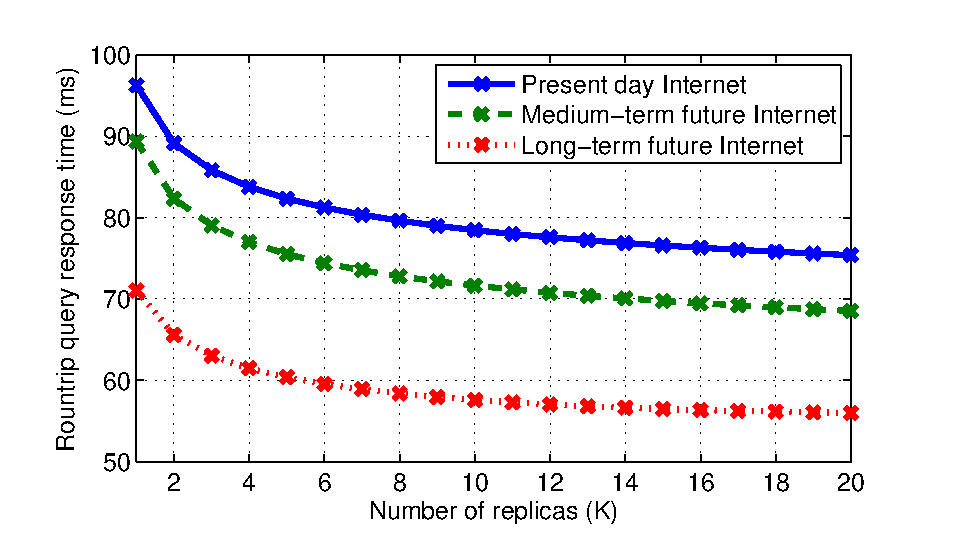
\includegraphics[width=0.5\textwidth]{figures/analysisUpperBound}
\caption{Analytical upper bound of query response times with the Internet topology evolution.}
\label{fig:resAnalysis}
\vspace{-0.2in}
\end{figure}
\end{center} 
%However there might be cases in which multiple tries are required for query resolution, which would increase the total response time from the derived estimates.
%\section{Discussion}
\label{sec:discussion}
We have so far presented the design of our ongoing work on naming resolution. In this section, we discuss opening problems and directions for our future works:

\paragraph{Different mapping schemes}
        Intuitively, our scheme relies on the fact that existing routing system dictate who handles which GUID to address mapping. However, it is noteworthy that our current approach which has GUID being distributed based on existing prefix table is only one of many design options. We can hash GUID directly to AS number as another option to equally distribute mapping over ASes without taking their announced prefix size into account.
        Another option could be hashing GUID to a predefined list of entities that registered to participate into the naming resolution service. This approach can address the incentive issues where only ASes that willing to participate into the service are assigned mapping. However, it also bring up additional overhead to our architecture, that is the cost to  maintain the membership of registered participants.
        We believe that there are many other options need to be investigated in depth to fully benefit our approach.

\paragraph{Caching scheme}
        While do not taking caching into the design as one of the primitive, we do recognize that the use of caching can further improve our fast lookup and update latency. However, selecting caching schemes should be taken with great caution since caching and mobility support always at the 2 end of the trade off. ***Mention few caching scheme with discussion in depth***[cite]


\paragraph{Biasing toward locality for better mapping distribution}
        Current approach has not taken requesters' demand into account. Instead, one of our design goals was equally distributed the mappings to ASes biasing to the size of address block that they announced. However, one extension could be taking the distribution of the original of the query into account while distributing mappings. For example, a mapping of a GUID belong to US should have at least one copy to be stored in a router in US.

\paragraph{Security issues due to the fact that we are relying on BGP table}
        Since our approach relies on available information of underlying routing infrastructure, security issues of the layer bellow might affect the reliability of our design. For example, to attack our service, attackers might announce many prefixes that they not actually own which leads to the inaccurate announced prefix table. However, there have been enormous amount of effort put toward securing routing layer cite[][]. For example, that kind of attack is not viable in newer version of BGP, SecureBGP, that under practical deployment plan....


\paragraph{Applicability of current scheme}
        Applicability of current scheme: We believe the naming resolution service is the center of the next generation Internet architecture, can find many applications beyond providing the mapping between host names and network addresses. As one example, it can facilitate efficient content retrieval. As a significant amount of content is produced and accessed by mobile devices, it is becoming an appealing approach to assign each content a global ID, and have the naming resolution service track the locations of each content file. As another example, it may also be useful to introduce the concept of contexts as the message recipients. An example of context can be ``all the cars in New Brunswick, NJ". In this case, the naming resolution service can be used to track which network addresses belong to a specific context.
\paragraph{Inconsistency in naming lookup result}
        Maintaining consistency among multiple replicas is very challenging, it at all possible. For example, one of the resolvers may be offline at an update. When it becomes back online later, it will contain stale information. In our system, we plan to adopt a weak consistency model, which we refer to as \emph{online update consistency}. Specifically, at each update, we only guarantee all the online resolvers will have the consistent view by employing the ACK mechanism. Our rationale is that, this consistency model can provide stronger consistency to hosts with frequent updates, which is a desirable feature. In our continuing work, we will work out a more thorough consistency model.
\paragraph{Incentive for participants or business model}
        [ Need more input ]


\vspace{-0.15in}
\section{Related Work}
\label{sec:related}
Given the importance of locator/identifier separation schemes in both current and future networks, various architectures for mapping identifiers to locators have been proposed and studied. Most of the early mapping schemes~\cite{farinacci-alt,jen,jakab,mathy} assumed aggregatable identifier spaces and proposed ideas based on that vantage point. However, this assumption is too restrictive making such schemes not applicable to many recent mainstream proposals such as HIP~\cite{moskowitz}, AIP~\cite{andersen} and MobilityFirst~\cite{mobilityFirst} which propose flat identifiers. Our approach, in contrast, targets a flexible resolution service by not making any assumptions about identifier hierarchy or locator structure.

There are some recent mapping architecture proposals that incorporate flat identifier space such as DHT-MAP~\cite{luo}, SLIMS~\cite{hou}. However these approaches either incur high lookup latency, making it not applicable to highly mobile environment, or high
management overhead which limits scalability. For example, the DHT based scheme in~\cite{luo} can entail up to 8 logical hops introducing an average latency of about 900ms as per their assumptions.

%While providing failure resilience and self-organizing property, DHT-based approaches may lead to excessive access delays due to multi-overlay-hop communication and management overhead.

In contrast, our scheme aims for much lower latencies by employing the one-hop hashing approach and ensures minimum management overhead for feasible deployment on a global scale. We argue that making use of network entities and the IP reachability information already available through the underlying routing infrastructure provides a practical and scalable approach to realize mapping resolvers. Reference~\cite{seattle_Kim} uses a similar in-network hashing scheme to target the different but related problem of name-based routing.

This work also focuses on a global-scale simulation to validate the design, which has been neglected in most of the prior works referenced above. Reference \cite{jakab} is a recent exception which presents a trace based simulation using the iPlane dataset~\cite{madhyastha}. Our simulation approach is more realistic than that of~\cite{jakab} on two counts: (a) We use a larger dataset from DIMES~\cite{shavitt} to extract AS level connectivity and latency information. The DIMES dataset is based on measurements from $\sim$1000 vantage points compared to $\sim$200 for iPlane, resulting in information for about twice the number of ASs as compared to iPlane; (b) To generate resolution lookup events,~\cite{jakab} uses DNS lookup traces from two particular source locations which introduces a significant locality bias in their results. In contrast, we globally distribute lookup source locations by weighting the chances of choosing a particular source location (source AS) in proportion to the available data on number of end nodes near that location. The basic intuition here is to mimic realistic deployment where more lookup requests will be generated from more densely populated areas.

%Existing schemes can be broadly categorized into two groups based on the identifier structure being assumed, namely \emph{aggregatable identifier}~\cite{farinacci-alt,jen,jakab,mathy} and \emph{flat identifier}~\cite{luo,hou}. In sharp contrast with the former group, our scheme is applicable to any any constraint moving away from a centralized control over name and address ownership, which forms a single root of global trust


%The key differences of our designs comparing to existing techniques are independence of identifier and locator structure, single-overlay-hop lookup and



%Seattle make use of

%DNS-based schemes where locator structure are assumed being hierarchical and DHT-based schemes in which a
%incur one (or more than one) of the following limitations: (i) identifier structure dependence, (ii) spaces or hierarchical underlying routing structure,
%One
%Our approach is moving away from a centralized control over name and address ownership, which forms a single root of global trust, to a fully distributed, hence highly scalable, scheme. \arcName~utilizes underlying routing infrastructure to create a network consisting of globally distributed nodes.

%Being a critical component of locator/identifier separation schemes, various architectures for mapping identifier to locator have been proposed and studied since the very introduction of these separation ideas. Most of the early separation schemes~\cite{farinacci-alt,jen,jakab,mathy} implicitly assumed aggregatable identifier spaces and hence the accompanying mapping architecture was designed to make use of this aggregation. However an increasing number of recent mainstream proposals such as HIP~\cite{moskowitz}, AIP~\cite{andersen} and MobilityFirst~\cite{mobilityFirst} argue for flat identifiers by pointing out its fundamental benefits and implementation feasibility. As such, some recent mapping architecture proposals such as DHT-MAP~\cite{luo}, SLIMS~\cite{hou} are designed to work with a flat identifier space, which is also a basic assumption in our scheme.

%    Based upon the trends witnessed by today's Internet, we believe an efficient global naming resolution service should have the following properties.
 %Firstly, it should be highly scalable be able to support billions of mobile devices.
 %Secondly, it should be responsive and provide access latencies as low as tens of milliseconds. Here, accesses include naming entry updates as well as lookups. *** why tens of ms? ***
 %Thirdly, it should be generic and independent of any specific naming structure.
  %Fourthly, it should be backward compatible with current Internet infrastructure.
  %Fifthly, it should be robust, and resilient against random node and network failures.

%Examples of mapping architectures for aggregatable identifiers include LISP-ALT~\cite{farinacci-alt}, which proposes an overlay scheme through which ETRs can broadcast their identifier prefixes globally similar to BGPs functionality, and APT~\cite{jen} which also relies on identifier aggregation to store the entire global mapping table at one or more ``default mappers" inside each AS. More recently, LISP-TREE~\cite{jakab} introduced a DNS based mapping architecture that uses increasing scopes of identifier prefixes to hierarchically arrange specialized mapping servers. In addition to being unfeasible for flat identifier structure, this scheme suffers from the fact that host mobility greatly reduces the effectiveness of any caching scheme, which in turn \emph{is} the main advantage of the DNS. LISP-DHT~\cite{mathy} proposes an opposite approach of arranging the mapping servers -  in a completely distributed manner and uses a Chord like overlay scheme to answer mapping queries. However the basic assumption that each resolver stores a continuous set of identifier mappings and using its highest value as the node identifier makes it particularly unsuited for flat identifiers.

%\cite{ahlgren} describes the key architectural challenges of mapping flat identifiers to locators and points out that while DHT based approaches are promising for local-scope resolution, the inherent problems of large average hop count and substantial overhead in case of churn inhibit its application for global-scope resolution. The DHT based scheme in ~\cite{luo}, for example, can entail up to 8 logical hops introducing an average latency of about 900ms as per the assumptions in~\cite{luo}. Our scheme, in contrast, aims for much lower latencies to ensure feasible deployment on a global scale. \cite{hou} describes an alternative probabilistic caching based scheme for flat identifiers but it requires significant management overhead for collecting flow information and making caching policies.

%A key focus of our project is also on detailed, global-scale validation of our proposal, which has been neglected in most of the prior works referenced above. \cite{jakab} is a recent exception which presents a trace based simulation using the iPlane dataset~\cite{madhyastha} for realistically modeling Internet topology and latencies. Our simulation approach differs from that of~\cite{jakab} on two main fronts: (a) We use the Dimes database~\cite{shavitt} for extracting AS level connectivity and latency graphs which relies on ~1000 vantage points compared to ~200 for iPlane and results in information for about twice the number of ASs as compared to iPlane; (b) To generate lookup requests,~\cite{jakab} uses DNS lookup traces from two particular source locations which might introduce a significant local bias on the resulting data. In contrast, we globally distribute lookup source locations by weighting the chances of choosing a particular source location (source AS) in proportion to the available data on number of end nodes near that location. The basic intuition here is to mimic realistic deployment where more lookup requests will be generated from more densely populated areas.

%Scalability of the current Internet routing protocol has been a core topic of discussion in the networking community in the recent past. While the timeline for expected large scale routing related performance issues have been debated, there is general consensus on the increasing inefficiency and lack of feature support in the existing IP routing protocol~\cite{narten}. Super-linear growth in the number of prefixes being propagated into the DFZ, increase in the rate of routing updates, increase in the demand for multi-homing support and intra-AS traffic engineering are some of the main contributors to this cause. A recent report from Internet Research Task Force - RFC 6115~\cite{li} summarizes the proposed approaches to tackle the scalability problems in the current architecture. Even though the group could not select a single proposal for endorsement, the group reached "rough consensus that separating identity from location is desirable and technically feasible." One of the key points of critique of the multiple proposals on locator-Identifier split architecture, listed in~\cite{li} was the feasibility of a scalable infrastructure for mapping from locator to identifier. In this paper, we explore precisely this topic and present the outline of a novel distributed mechanism for resolving the locator to identifier mappings.
%The Locator/ID Separation Protocol~\cite{farinacci} and other similar proposals [?,?] address the problem associated with using a single namespace, the IP address, to simultaneously express two functions about a device. Instead they propose two different namespaces - an endpoint identifier (EID), which serves as the device identity and a routing locator (RLOC) which denotes its network location.\\

%TBA: detail about LISP\\
%TBA: mention MobilityFirst and how this fits\\

\section{Concluding Remarks}
\label{sec:conclusion}
In this paper, we presented the concept, design and evaluation of DMap, a scheme for low latency, scalable name resolution service in the future Internet. DMap distributes name to address mappings amongst Internet routers using an in-network single-hop hashing technique that derives the address of the storage router directly from a flat, globally unique identifier. In contrast to other DHT-based techniques, DMap does not require any table maintenance overhead since we use network level reachability information already available through existing routing protocols. In addition, DMap supports arbitrary name and address structures making it more widely applicable than prior techniques. Through a large-scale discrete-event simulation, we show that the proposed DMap method achieves low latencies with a mean value of $\sim$50 ms and 95th percentile value of $\sim$100 ms and good storage distribution among participating routers.

In further work, we plan to consider other variations of the proposed DMap distribution scheme - for example GUIDs can be hashed directly to AS numbers or allocation sizes can be varied to reflect economic incentives at ASs. We also plan to extend the scope of this work by studying a feasible in-network caching methods that builds on top of the basic DMap scheme. Since our scheme interacts with the hosts, the inter-domain routing protocol and the Internet routers, security is a critical requirement at each level. The MobilityFirst project~\cite{mobilityFirst}, takes a holistic approach towards self certification based security, which tie in well into the relevant aspects of our scheme. Our future work plan also includes incorporating the transient effects of BGP updates, misconfigurations and router failures.

On the validation and evaluation front, there is an ongoing effort to implement a proof-of-concept global scale DMap system using the GENI (global environment for network innovation) framework.  A first DMap prototype was demonstrated at the GENI Engineering Conference-12 in Kansas City and efforts are currently under way to fully instrument the latency and overhead measurements necessary to evaluate scalability and performance.  If the GENI experiments successfully confirm DMap performance, there are also further plans to use the proposed technique as part of a complete identifier-based protocol stack in the MobilityFirst future Internet architecture project.


 
\section*{Acknowledgements}
We would like to thank Jennifer Rexford for her insightful comments. We also thank Noa Zilberman and Udi Weinsberg from DIMES for their help with the latency dataset. 


{\scriptsize
\bibliographystyle{IEEEtran}
\bibliography{paper}
}

%{\scriptsize
%	\bibliographystyle{abbrv}
%	\bibliography{paper}
%}

\end{document}
